\documentclass[leqno, openany]{memoir}
\setulmarginsandblock{3.5cm}{3.5cm}{*}
\setlrmarginsandblock{3cm}{3.5cm}{*}
\checkandfixthelayout

\usepackage{amsmath}
\usepackage{amssymb}
\usepackage{amsthm}
%\usepackage{MnSymbol}
\usepackage{bm}
\usepackage{accents}
\usepackage{mathtools}
\usepackage{tikz}
\usepackage{pgfplots}
\usetikzlibrary{calc}
\usetikzlibrary{automata,positioning}
\usepackage{tikz-cd}
\usepackage{forest}
\usepackage{braket} 
\usepackage{listings}
\usepackage{mdframed}
\usepackage{verbatim}
\usepackage{physics}
\usepackage{tkz-euclide}
%\usepackage{/home/patrickl/homework/macaulay2}

%font
\usepackage{mathpazo} 
\usepackage{microtype}

%CS packages
\usepackage{algorithmicx}
\usepackage{algpseudocode}
\usepackage{algorithm}

% typeset and bib
\usepackage[english]{babel} 
\usepackage[utf8]{inputenc} 
\usepackage[backend=biber, style=alphabetic]{biblatex}
\usepackage[bookmarks, colorlinks, breaklinks]{hyperref} 
\hypersetup{linkcolor=black,citecolor=black,filecolor=black,urlcolor=black}

% other formatting packages
\usepackage{float}
\usepackage{booktabs}
\usepackage{enumitem}
\usepackage{csquotes}
\usepackage{titlesec}
\usepackage{titling}
\usepackage{fancyhdr}
\usepackage{lastpage}
\usepackage{parskip}

\usepackage{lipsum}

% delimiters
\DeclarePairedDelimiter{\gen}{\langle}{\rangle}
\DeclarePairedDelimiter{\floor}{\lfloor}{\rfloor}
\DeclarePairedDelimiter{\ceil}{\lceil}{\rceil}


\newtheorem{thm}{Theorem}[section]
\newtheorem{cor}[thm]{Corollary}
\newtheorem{prop}[thm]{Proposition}
\newtheorem{lem}[thm]{Lemma}
\newtheorem{conj}[thm]{Conjecture}
\newtheorem{quest}[thm]{Question}
\newtheorem{prob}[thm]{Problem}

\theoremstyle{definition}
\newtheorem{defn}[thm]{Definition}
\newtheorem{defns}[thm]{Definitions}
\newtheorem{con}[thm]{Construction}
\newtheorem{exm}[thm]{Example}
\newtheorem{exms}[thm]{Examples}
\newtheorem{notn}[thm]{Notation}
\newtheorem{notns}[thm]{Notations}
\newtheorem{addm}[thm]{Addendum}
\newtheorem{exer}[thm]{Exercise}

\theoremstyle{remark}
\newtheorem{rmk}[thm]{Remark}
\newtheorem{rmks}[thm]{Remarks}
\newtheorem{warn}[thm]{Warning}
\newtheorem{sch}[thm]{Scholium}


% unnumbered theorems
\theoremstyle{plain}
\newtheorem*{thm*}{Theorem}
\newtheorem*{prop*}{Proposition}
\newtheorem*{lem*}{Lemma}
\newtheorem*{cor*}{Corollary}
\newtheorem*{conj*}{Conjecture}

% unnumbered definitions
\theoremstyle{definition}
\newtheorem*{defn*}{Definition}
\newtheorem*{exer*}{Exercise}
\newtheorem*{defns*}{Definitions}
\newtheorem*{con*}{Construction}
\newtheorem*{exm*}{Example}
\newtheorem*{exms*}{Examples}
\newtheorem*{notn*}{Notation}
\newtheorem*{notns*}{Notations}
\newtheorem*{addm*}{Addendum}


\theoremstyle{remark}
\newtheorem*{rmk*}{Remark}

% shortcuts
\newcommand{\Ima}{\mathrm{Im}}
\newcommand{\A}{\mathbb{A}}
\newcommand{\R}{\mathbb{R}}
\newcommand{\C}{\mathbb{C}}
\newcommand{\Z}{\mathbb{Z}}
\newcommand{\Q}{\mathbb{Q}}
\newcommand{\N}{\mathbb{N}}
\renewcommand{\k}{\Bbbk}
\renewcommand{\P}{\mathbb{P}}
\newcommand{\M}{\overline{M}}
\newcommand{\g}{\mathfrak{g}}
\newcommand{\h}{\mathfrak{h}}
\newcommand{\n}{\mathfrak{n}}
\renewcommand{\b}{\mathfrak{b}}
\newcommand{\ep}{\varepsilon}
\newcommand*{\dt}[1]{%
   \accentset{\mbox{\Huge\bfseries .}}{#1}}
\renewcommand{\abstractname}{Official Description}
\newcommand{\mc}[1]{\mathcal{#1}}
\newcommand{\T}{\mathbb{T}}
\newcommand{\mf}[1]{\mathfrak{#1}}
\newcommand{\mr}[1]{\mathrm{#1}}
\newcommand{\ol}[1]{\overline{#1}}
\newcommand{\wt}[1]{\widetilde{#1}}


\DeclareMathOperator{\Der}{Der}
\DeclareMathOperator{\Hom}{Hom}
\DeclareMathOperator{\End}{End}
\DeclareMathOperator{\ad}{ad}
\DeclareMathOperator{\Aut}{Aut}
\DeclareMathOperator{\Rad}{Rad}
\DeclareMathOperator{\supp}{supp}
\DeclareMathOperator{\sgn}{sgn}
\DeclareMathOperator{\len}{length}

% Section formatting
\titleformat{\section}
    {\Large\sffamily\scshape\bfseries}{\thesection}{1em}{}
\titleformat{\subsection}[runin]
    {\large\sffamily\bfseries}{\thesubsection}{1em}{}
\titleformat{\subsubsection}[runin]{\normalfont\itshape}{\thesubsubsection}{1em}{}

\title{COURSE TITLE}
\author{Lectures by INSTRUCTOR, Notes by NOTETAKER}
\date{SEMESTER}

\newcommand*{\titleSW}
    {\begingroup% Story of Writing
    \raggedleft
    \vspace*{\baselineskip}
    {\Huge\itshape Complex Analysis \\ Math 621}\\[\baselineskip]
    {\large\itshape Notes by Patrick Lei,
                    June 2020}\\[0.2\textheight]
    {\Large Lectures by Paul Hacking, Spring 2018}\par
    \vfill
    {\Large \sffamily University of Massachusetts Amherst}
    \vspace*{\baselineskip}
\endgroup}
\pagestyle{simple}

\chapterstyle{ell}


%\renewcommand{\cftchapterpagefont}{}
\renewcommand\cftchapterfont{\sffamily}
\renewcommand\cftsectionfont{\scshape}
\renewcommand*{\cftchapterleader}{}
\renewcommand*{\cftsectionleader}{}
\renewcommand*{\cftsubsectionleader}{}
\renewcommand*{\cftchapterformatpnum}[1]{~\textbullet~#1}
\renewcommand*{\cftsectionformatpnum}[1]{~\textbullet~#1}
\renewcommand*{\cftsubsectionformatpnum}[1]{~\textbullet~#1}
\renewcommand{\cftchapterafterpnum}{\cftparfillskip}
\renewcommand{\cftsectionafterpnum}{\cftparfillskip}
\renewcommand{\cftsubsectionafterpnum}{\cftparfillskip}
\setrmarg{3.55em plus 1fil}
\setsecnumdepth{subsection}
\maxsecnumdepth{subsection}
\settocdepth{subsection}

\begin{document}
    
\begin{titlingpage}
\titleSW
\end{titlingpage}

\thispagestyle{empty}
\section*{Disclaimer}%
\label{sec:disclaimer}

These notes are a transcription of handwritten notes that were taken during lecture. 
Any errors are mine and not the instructor's. 
In addition, my notes are picture-free (but will include commutative diagrams) and are a mix of my mathematical style 
(omit lengthy computations, use category theory) and that of the instructor.
If you find any errors, please contact me at \texttt{plei@umass.edu}.
\newpage

\tableofcontents

\chapter{Basic Notions}%
\label{cha:basic_notions}

A \textit{complex number} is a sum $z = x + iy$, where $x,y \in \R$ and $i$ is a symbol satisfying the identity $i^2 = -1$. Addition and multiplication work as one would expect. The set $\C$ of complex numbers is a \textit{field}. This means that $(\C,+)$ is an abelian group, $(\C \setminus \qty{0}, \cdot)$ is an abelian group, and that multiplication distributes over addition.

\begin{rmk}
    If $F$ is a field and $f \in F[x]$ is irreducible, then we can construct a field extension $K/F$ such that $K$ has a root of $f$ by setting $K = F[x]/(f)$. In this way, we have $\C = \R[x] / (x^2 + 1)$. The Galois group $\operatorname{Gal} \C/\R$ is generated by complex conjugation.
\end{rmk}

\section{Holomorphic Functions}%
\label{sec:holomorphic_functions}

Let $\Omega \subset \C$ be an open set. Here, the topology is the Euclidean topology on $\C = \R^2$. Then $f: \Omega \to \C$ is \textit{holomorphic} at a point $z_0 \in \Omega$ if the limit
\[ \lim_{h \to 0} \frac{f(z_0+h) - f(z_0)}{h} \]
exists. If it does, we write $f'(z_0)$ for the derivative at $z_0$.

\begin{exm}
    The function $f(z) = \ol{z}$ is \textbf{not} holomorphic. To see this, the difference quotient has different limits on the real and imaginary axes.
\end{exm}

\begin{exm}
    The function $f(z) = z^n$ is holomorphic for $n \in \N$, and $f'(z) = nz^{n-1}$.
\end{exm}

\begin{rmk}
    The usual formulas for differentiation (chain rule, product rule, linearity) hold in this case.
\end{rmk}

We will now compare holomorphic and real differentiability. Rewrite $F = u + iv$. Recall that $F$ is \textit{real differentiable} at $\mathbf{a} = (x_0,y_0)$ if 
\[ \lim_{\mathbf{h} \to 0} \frac{\norm{F(\mathbf{a} + \mathbf{h}) - F(\mathbf{a}) - A \mathbf{h}}}{\norm{\mathbf{h}}} = 0 \]
for some linear map $A$. We say that $A$ is the derivative of $F$ at $\mathbf{a}$. Moreover, $A$ is given by the \textit{Jacobian matrix}
\[ J_F = \begin{pmatrix}
    \pdv{u}{x} & \pdv{u}{y} \\
    \pdv{v}{x} & \pdv{v}{y}
\end{pmatrix}. \]
Note that $F$ is differentiable if and only if the partials exist and are continuous. Then recalling that holomorphic means that 
\[ \lim_{h \to 0} \frac{f(z_0 + h) = f(z_0) - f'(z_0)h}{h} = 0, \]
we see that $f$ is holomorphic if and only if $f$ is differentiable and $J_{Z_0} F$ corresponds to multiplication by a complex number.

\begin{rmk}
    The standard definition of holomorphic is that the differentiability condition is satisfied in an open neighborhood around $z_0$.
\end{rmk}

Now recall that if $\lambda = a+ib \in \C$, multiplication by $\lambda$ is given by the real matrix $\begin{psmallmatrix} a & -b \\ b & a \end{psmallmatrix}$. Therefore, we must have $u_x = v_y$ and $u_y = -v_x$. These are the \textit{Cauchy-Riemann equations}. 

\begin{thm}[Cauchy-Riemann]
    The function $f \colon U \to \C$ is holomorphic if and only if it is real differentiable and its Jacobian satisfies the Cauchy-Riemann equations.
\end{thm}

We can also write $\lambda = r(\cos \theta + i \sin\theta) = re^{i\theta} \in \C$ in polar form. We know that multiplication by $\lambda$ is rotation by $\theta$ followed by dilation by $r$, so in particular it preserves angles. Suppose $f \colon U \to \C$ is holomorphic at $z_0$ and $\gamma_1, \gamma_2 \colon (-1,1) \to U$ are parameterized curve with $\gamma_i(0) = z_0$, then we define the angle between $\gamma_1, \gamma_2$ to be the angle between $\gamma_1'(0)$ and $\gamma_2'(0)$. We also obtain the curves $f \gamma_1, f \gamma_2$. If $f'(z_0 \neq 0)$, then the angle between $f \gamma_1, f\gamma_2$ equals the angle between $\gamma_1, \gamma_2$. To see this, the chain rule gives us
\[ {(f \gamma_i)}'(0) = f'(\gamma_i(0)) \gamma_i'(0) = f'(z_0) \gamma_i'(0). \]
\begin{rmk}
    Note that the condition that $f'(z_0) \neq 0$ is necessary. In fact, $f$ is conformal at $z_0$ if and only if $f'(z_0) \neq 0$. For example, consider $f(z) = z^2$, which satisfies $f'(0) = 0$.
\end{rmk}

\section{Power Series}%
\label{sec:power_series}

\begin{thm}
    Let $\sum_{n=0}^{\infty} a_n z^n$ be a power series with $a_n \in \C$. Then there exists $R \in R_{\geq 0} \cup \infty$ such that
    \begin{enumerate}
        \item The series converges absolutely for $\abs{z} < R$;
        \item The series diverges for $\abs{z} > r$.
    \end{enumerate}
    Moreover, we have $\frac{1}{R} = \limsup_{n \to \infty} \abs{a_n}^{1/n}$.
\end{thm}

Recall that if $b_n$ is a sequence of real numbers, we define
\[ \limsup b_n = \lim_{m \to \infty} \sup_{n \geq m} b_n. \]
This exists if $b_n$ is bounded below because the sequence of supremums is decreasing.

\begin{proof}
    Define $R$ by the formula. Given $\ep > 0$, there exists $N \in \N$ such that $\abs{a_n}^{1/n} \leq \frac{1}{R} + \ep$ for $n > N$. Then 
    \[ \abs{a_n z^n} = {(\abs{a_n}^{1/n} \abs{z})}^{n} < {\qty( \qty(\frac{1}{R} + \ep) \abs{z} )}^n, \]
    so if $\abs{z} < \frac{1}{\frac{1}{R} + \ep}$, then the series converges absolutely by the comparison test. Then $\ep$ is arbitrary, so the series converges absolutely for $\abs{z} < R$.

    If $\abs{z} > R$, then fix $\rho$ such that $\abs{z} > \rho > R$. For all $N \in \abs{N}$, there exists $n > N$ such that $\abs{a_n}^{1/n} > \frac{1}{\rho}$. Now 
    \[ \abs{a_n z^n} > \qty(\frac{\abs{z}}{\rho})^n \to \infty \]
    as $n \to \infty$, because $\frac{\abs{z}}{\rho} > 1$.
\end{proof}

\begin{thm}
    Let $f(z) = \sum_{n=0}^{\infty} a_n z^n \in \C[[z]]$ have radius of convergence $R$ and $\Omega = \qty{z \mid \abs{z} < R}$. Then $f \colon \Omega \to C$ is holomorphic and $f'(z) = \sum_{n=1}^{\infty} n a_n z^{n-1}$ has the same radius of convergence.
\end{thm}

Here is the most important example of a power series.
\begin{exm}
    Define $e^z - \sum_{n = 0}^{\infty} \frac{z^n}{n!}$. This has radius of convergence $R = \infty$ because 
    \[ \frac{1}{R} = \limsup_{n \to \infty} {\qty(\frac{1}{n!})}^{1/n} \geq \limsup_{n \to \infty} {\qty(\frac{n}{2})}^{1/2} = \infty. \]
    Alternatively, we may use the ratio test instead of the root test.
\end{exm}

It is easy to see that $\dv{z} e^z = e^z$ from the power series. Then we have
\begin{align*}
    e^{z+w} &= \sum_{n=0}^{\infty} \frac{{(z+w)}^n}{n!} \\
            &= \sum_{n=0}^{\infty} \frac{1}{n!} \sum_{k=0}^n \binom{n}{k} z^k w^{n-k} \\
            &= \sum_{n=0}^{\infty} \sum_{k=0}^{n} \frac{z^k}{k!} \frac{w^{n-k}}{(n-k)!} \\
            &= \qty(\sum_{k=0}^{\infty} \frac{z^k}{k!}) \qty(\sum_{\ell = 0}^{\infty} \frac{w^{\ell}}{\ell!}) \\
            &= e^z e^w
\end{align*}
because if $\sum a_n, \sum b_n$ are absolutely convergent and $c_n = \sum_{k=0}^n a_k b_{n-k}$, then $\sum c_n$ is absolutely convergent and $\sum c_n = \sum a_n \cdot \sum b_n$ (see baby Rudin for a reference).

Now we may define
\begin{align*}
    \cos z &= \sum_{n=0}^{\infty} {(-1)}^n \frac{z^{2n}}{(2n)!} = \frac{e^{iz} + e^{-iz}}{2} \\
    \sin z &= \sum_{n=0}^{\infty} {(-1)}^n \frac{z^{2n+1}}{(2n+1)!} = \frac{e^{iz} - e^{-iz}}{2i}.
\end{align*}
It is easy to see from the power series that $e^{\pm iz} = \cos z \pm i \sin z$. The formulas for the derivatives from basic calculus hold.

\begin{exm}
    Consider the series $\sum_{n=0}^{\infty} z^n$. This has radius of convergence $R = 1$ and diverges for $\abs{z} \geq 1$. In fact, $f(z) = \frac{1}{1-z}$ for $\abs{z} < 1$. In this case, the power series $f(z)$ extends to a holomorphic $g(z) = \frac{1}{1-z}$ defined on $\C \setminus \qty{1}$. More generally, if $g \colon \Omega \to C$ is holomorphic and $z_0 \in \Omega$ is a point, then it has a power series expansion 
    \[ g(z) = \sum_{n=0}^{\infty} \frac{g^{(n)}(z_0) {(z-z_0)}^n}{n!} \]
    valid in the largest open disc contained in $\Omega$. This means that $g$ is an \textit{analytic continuation} of $f$. 
\end{exm}

Note that convergence for $\abs{z} = R$ is very delicate.
\begin{enumerate}
    \item The series $\sum z^n$ has $R = 1$ and diverges when $\abs{z} = 1$;
    \item The series $\sum \frac{1}{n^2} z^n$ has $R = 1$ and converges absolutely for $\abs{z} = 1$;
    \item The series $\sum \frac{1}{n} z^n$ has $R = 1$ and diverges for $z = 1$ but converges for $\abs{z} = 1, z \neq 1$.
\end{enumerate}

\section{Integration along curves}%
\label{sec:integration_along_curves}

A \textit{paramaterized curve} is a continuous function $z \colon [a,b] \to \C$. We will call it \textit{smooth} if $z$ is continuously differentiable. We also assume that $z'(t) \neq 0$ for all $t \in [a,b]$.

\begin{exm}
    The circle centered at $z_0$ with radius $r$ is given by
    \[ z \colon [0, 2\pi] \to \C \qquad z(t) = z_0 + re^{it} = z_0 + r (\cos t + i \sin t). \]
\end{exm}
Two parameterized curves $z_1 \colon [a,b] \to \C, z_2 \colon [c,d] \to \C$ are \textit{equivalent} if there exists a $C^1$ homeomorphism $t \colon [c,d] \to [a,b]$ with $t'(s) = 0$ for all $s \in [c,d]$ and $z_2 = z_1 \circ t$. Therefore, we can define a \textit{smooth curve} to be an equivalence class of parameterized curves. It is \textit{closed} if $z(a) = z(b)$ and simple if $z(s) \neq z(t)$ for all $s \neq t$ unless $s,t = a,b$. Given a curve $\gamma$ with parameterization $z \colon [a,b] \to \C$, we write $-\gamma$ for the curve
\[ \wt{z} \colon [a,b] \to \C \qquad t \mapsto z(a+b-t). \]

We may finally define integration along a curve. If $f$ is continuous and $\gamma$ is a smooth curve, we define
\[ \int_{\gamma} f(z) \dd{z} \coloneqq \int_a^b f(z(t)) z'(t) \dd{t} \]
for some parameterization $z \colon [a,b] \to \C$ of $\gamma$. We need to check that this is well-defined, and we have
\begin{align*}
    \int_a^b f(z_1(t)) z_1'(t) &= \int_c^d f(z_1(t(s))) z_1'(t(s)) t'(s) \dd{s} \\
                               &= \int_c^d f(z_2(s)) z_2'(s).
\end{align*}

\begin{exm}
    Let $\gamma$ be a circle of radius $r$ centered at the origin with parameterization $z \colon [0,2\pi] \to \C$ given by $z(t) = re^{it}$. Then we have
    \[ \int_{\gamma} \frac{1}{z} \dd{z} = \int_0^{2 \pi} \frac{1}{re^{it}} {(re^{it})}' = \int_0^{2 \pi} \frac{1}{re^{it}} ire^{it} \dd{t} = 2 \pi i. \]
\end{exm}

It is easy to see that $\int_{- \gamma} f(z) \dd{z} = - \int_{\gamma} f(z) \dd{z}$. We may also define the length
\[ \len(\gamma) \coloneqq \int_a^b \abs{z'(t)} \dd{t} = \int_a^b \sqrt{ {x'(t)}^2 + {y'(t)}^2 } \dd{t}. \]
This has an easy bound given by
\[ \abs{ \int_a^b f(z(t)) z'(t) \dd{t} } \leq \int_a^b \abs{f(z(t))} \abs{z'(t)} \dd{t} \leq \sup_{z \in \gamma} \abs{f(z)} \int_a^b \abs{z'(t)} \dd{t} = \sup_{z \in \gamma} \abs{f(z)} \cdot \len(\gamma). \]

\begin{thm}[Fundamental Theorem of Calculus]
    Let $f \colon \Omega \to \C$ be continuous ans assume there exists a holomorphic $F \colon \Omega \to \C$ such that $F' = f$ (in other words, a \textit{primitive} for $f$). Then 
    \[ \int_{\gamma} f(z) \dd{z} = F(z(b)) - F(z(a)). \]
    In particular, if $\gamma$ is closed, then $\int_{\gamma} f(z) \dd{z} = 0$.
\end{thm}

\begin{proof}
    By definition, we have 
    \begin{align*}
        \int_{\gamma} f(z) \dd{z} &= \int_a^b f(z(t)) z'(t) \dd{t} \\
                                  &= \int_a^b F'(z(t)) z'(t) \dd{t} \\
                                  &= \int_a^b {(F \circ z)}'(t) \dd{t} \\
                                  &= F(z(b)) - F(z(a))
    \end{align*}
    by the fundamental theorem of calculus over $\R$.
\end{proof}

\chapter{Local Theory}%
\label{cha:local_theory}

\section{Integrals of Holomorphic Functions}%
\label{sec:integrals_of_holomorphic_functions}

\begin{thm}[Cauchy]
    Let $f \colon \Omega \to \C$ be holomorphic and $\gamma$ be a simple closed curve in $\Omega$ such that the interior of $\gamma$ is contained in $\Omega$. Then
    \[ \int_{\gamma} f(z) \dd{z} = 0. \]
\end{thm}

\begin{warn}
    It is very tricky to precisely describe what is meant by ``interior'' and we need the Jordan curve theorem from algebraic topology to do so.
\end{warn}

\begin{proof}[Sketch of Proof]
    We write
    \begin{align*}
        \int_{\gamma} f(z) \dd{z} &= \int_{\gamma} (u+iv) (\dd{x} + i \dd{y}) \\
                                  &= \int_{\gamma} u \dd{x} - v \dd{y} + i \int_{\gamma} v \dd{x} + u \dd{y} \\
                                  &= \int_R \qty(\pdv{v}{x} - \pdv{u}{y}) \dd{x} \dd{y} + i \int_{\gamma} \qty(\pdv{u}{x} - \pdv{v}{y}) \dd{x} \dd{y} \\
                                  &= 0
    \end{align*}
    by Green's theorem and the Cauchy-Riemann equations.
\end{proof}

Of course, this assumes that the partial derivatives of $u,v$ are $C^{\infty}$, which we do not know yet. Instead, we will give a more careful proof of a weaker theorem.

\begin{thm}[Goursat]
    Let $f \colon \Omega \to \C$ be holomorphic and $T \subset \Omega$ be a triangle. Then 
    \[ \int_{\partial T} f(z) \dd{z} = 0. \]
\end{thm}

\begin{proof}
    Bisect each side of $T$ and create four smaller triangles $T_i^1$. Then we have
    \[ \int_{\partial T} f(z) \dd{z} = \sum_{i=1}^4 \int_{\partial T_i^1} f(z) \dd{z} \]
    and thus 
    \[ \abs{\int_{\partial T} f(z) \dd{z}} \leq 4 \abs{\int_{\partial T_i^1} f(z) \dd{z}} \]
    for some $i$. Now write $T^1 = T_i^1$. We may repeat this process to obtain
    \[ T \supset T^1 \supset T^2 \supset \cdots \supset T^n \supset \cdots, \]
    and thus we have
    \[ \abs{\int_{\partial T} f(z) \dd{z}} \leq 4^n \abs{\int_{\partial T^n} f(z) \dd{z}} \]
    and $\len(\partial T^n) = 2^{-n} \len(\partial T)$. Now set $z_0 = \bigcap_{n \geq 1} T^n$. We now use the holomorphicity of $f$ to estimate the integral, and we have $f(z_0 + h) = f(z_0) + hf'(z_0) + h \psi(h)$, where $\lim_{h \to 0} \psi(h) = 0$. Therefore
    \begin{align*}
        \abs{\int_{\partial T^n} f(z) \dd{z}} &= \abs{\int_{\partial T^n} f(z_0) + (z-z_0)f'(z_0) + (z-z_0) \psi(z-z_0) \dd{z}} \\
                                              &= \abs{\int_{\partial T^n} (z-z_0) \psi(z-z_0) \dd{z}} \\
                                              &\leq \len(\partial T^n) \cdot \sup_{z \in \partial T^n} \abs{z-z_0}{\psi(z-z_0)} \\
                                              &\leq {\len(\partial T^n)}^2 \sup_{z \in \partial T^n} \abs{\psi(z-z_0)}.
    \end{align*}
    Therefore, we have
    \[ \abs{\int_{\partial T} f(z) \dd{z}} \leq 4^n {(2^{-n} \len(\partial T^n))} \sup_{z \in \partial T^n} \abs{\psi(z-z_0)} \to 0 \]
    as $n \to \infty$.
\end{proof}

\begin{cor}
    The same result holds for a rectangle.
\end{cor}

Now we want to discuss the existence of local primitives.

\begin{prop}
    Let $f \colon D \to \C$ be holomorphic on an open disc $D = D_r(z_0)$. Then there exists $F \colon D \to \C$ holomorphic such that $F' = f$. In particular, $\int_{\gamma} f(z) \dd{z} = 0$ for any closed curve $\gamma \subset D$.
\end{prop}

\begin{proof}
    Define $F$ as an integral
    \[ F(z) = \int_{\gamma_z} f(w) \dd{w}. \]
    Here, we define $\gamma_z$ as
    \begin{figure}[H]
    \begin{center}
    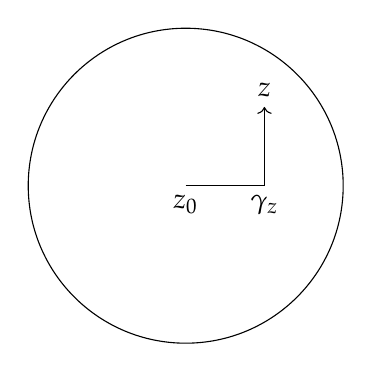
\begin{tikzpicture}[scale=1, transform shape]
        \draw[->] (0,0) node[align=left,below] {$z_0$}
            -- (1,0) node[align=right,below] {$\gamma_z$}
            -- (1,1) node[align=right,above] {$z$};
        \draw (0,0) circle [radius=2];
    \end{tikzpicture}
    \end{center}
    \caption{Path of integration}%
    \label{fig:}
    \end{figure}
    Now we need to prove that $F'(z) = f(z)$. Note that
    \[ F(z+h) - F(z) = \int_{\gamma_{z+h}} f(w) \dd{w} - \int_{\gamma_z} f(w) \dd{w}. \]
    Then note that the path of integration is given by
    \begin{figure}[H]
    \begin{center}
    \begin{tikzpicture}[scale=1, transform shape]
        \draw[-] (2,2) node[above left] {$z$} 
            -- (2,0) node {} 
            -- (0,0) node {}
            -- (3,0) node {} 
            -- (3,3) node[above right] {$z+h$};
        \draw[->] (1.8,1.2) -- (1.8,0.8);
        \draw[->] (1.2,0.2) -- (0.8,0.2);
        \draw[->] (0.8,-0.2) -- (1.2,-0.2);
        \draw[->] (3.2,1.3) -- (3.2,1.7);
        \node (A) at (4,1.5) {$\equiv$};
        \draw[->] (5,2) node[above left] {$z$} 
            -- (5,0) node {} 
            -- (6,0) node {} 
            -- (6,3) node[above right] {$z+h$};
        \node (B) at (7,1.5) {$\equiv$};
        \draw[->] (8,2) node[below left] {$z$} 
            -- (9,3) node[above right] {$z+h$};
    \end{tikzpicture}
    \end{center}
    \caption{Equivalent paths}%
    \label{fig:}
    \end{figure}
    Call the final path $[z,z+h]$. Therefore, 
    \begin{align*}
        F(z+h) - F(z) &= \int_{[z,z+h]} f(w) \dd{w} \\
                      &= \int_{[z,z+h]} (f(z) + \psi(w-z)) \dd{w} \\
                      &= f(z) \cdot h \int_{[z,z+h]} \psi(w-z) \dd{w},
    \end{align*}
    so
    \[ F'(z) = f(z) + \lim_{h \to 0} \frac{1}{h} \int_{[z,z+h]} \psi(w-z) \dd{w}, \]
    but then
    \[ \abs{\frac{1}{h} \int_{[z,z+h]} \psi(w-z) \dd{w}} \leq \abs{\frac{1}{h}} \abs{h} \sup_{w \in [z,z+h]} \abs{\psi(w-z)} \to 0 \]
    as $h \to 0$.
\end{proof}

Now we will relate the function $f$ itself to some integral of points neearby $f$.

\begin{thm}[Cauchy integral formula]
    Let $f \colon \Omega \to \C$ be holomorphic and $D$ be an open disc such that $\ol{D} \subset \Omega$. Then
    \[ f(z) = \frac{1}{2 \pi i} \int_{\partial D} \frac{f(w)}{w-z} \dd{w} \]
    for all $z \in D$.
\end{thm}

\begin{proof}
    First, if $\Omega'$ is a disk with a segment of a radius removed, then any holomorphic $f$ has a primitive on $\Omega'$ by the same argument as before. Now define the path $\gamma_{\ep, \delta}$ by
    \begin{figure}[H]
    \begin{center}
    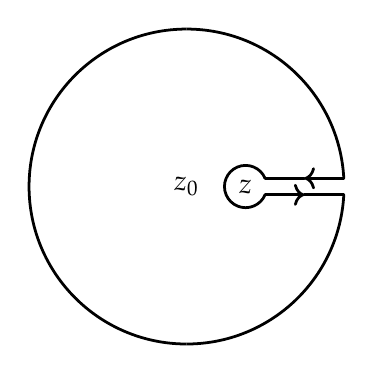
\begin{tikzpicture}[scale=1, transform shape]
        \tkzInit[xmin=-5,ymin=-5,xmax=5,ymax=5]
        \tkzDefPoint(0,0){O}
        \tkzDefPoint(0.75,0){P}
        \tkzDefPoint(3:2){D} \tkzDefPoint(90:2){M} \tkzDefPoint(270:2){N}
        \tkzDefPoint(-3:2){E}
        \tkzDefPoint[shift={(-1,0)}](3:2){B} \tkzDefMidPoint(B,D) \tkzGetPoint{B'}
        \tkzDefPoint[shift={(-1,0)}](-3:2){C} \tkzDefMidPoint(C,E) \tkzGetPoint{C'}

        \tkzDrawArc[color=black,line width=1pt](O,N)(E) 
        \tkzDrawArc[color=black,line width=1pt](P,B)(C)
        \tikzset{compass style/.append style={->}}
        \tkzDrawArc[color=black,line width=1pt](O,D)(M) 
        \tkzDrawArc[color=black,line width=1pt](O,M)(N) 

        \tkzDrawSegments[color=black,line width=1pt,->](D,B' C,C')
        \tkzDrawSegments[color=black,line width=1pt](B',B C',E)
        \node at (0,0) {$z_0$};
        \node at (0.75,0) {$z$};
    \end{tikzpicture}
    \end{center}
    \caption{Contour $\gamma_{\ep, \delta}$}%
    \label{fig:}
    \end{figure}
    where the radius of the circle around $z$ is $\delta$ and the width of the corridor is $2\ep$. Now $\frac{f(z)}{z-2}$ is holomorphic on the interior of $\gamma_{\ep, \delta}$, so there eixists a primitive. Therefore, $\int_{\gamma_{\ep, \delta}} \frac{f(w)}{w-z} \dd{z} = 0$. Now we let $\ep \to 0$. Because $\frac{f(w)}{w-z}$ is continuous on the rectangular corridor, we have 
    \[ \int_{\gamma_{\ep, \delta}} \frac{f(w)}{w-z} \dd{w} \to \int_{\gamma_{\delta}} \frac{f(w)}{w-z} \dd{w} \] 
    as $\ep \to 0$. This is because if $f$ is continuous on some rectangle, then
    \[ \int_a^b f(s,t) \dd{t} \to \int_a^b f(s_0, t) \dd{t} \]
    as $s \to s_0$ by uniform continuity on compact sets. Now we see that
    \[ 0 = \int_{\gamma_{\delta}} \frac{f(w)}{z-w} \dd{w} = \int_{\partial D} \frac{f(w)}{z-w} \dd{w} - \int_{\alpha_{\delta}} \frac{f(w)}{z-w} \dd{w}, \]
    where $\alpha_{\delta}$ is the circle of radius $\delta$ centered at $z$. Then we can rewrite
    \[ \frac{f(w)}{w-z} = \frac{f(z)}{w-z} + \frac{f(w) - f(z)}{w-z}, \]
    and the last term approaches $f'(z)$ as $w \to z$. Therefore it is bounded, so
    \[ \int_{\alpha_{\delta}} \frac{f(w) - f(z)}{w-z} \dd{w} \to 0 \]
    as $\delta \to 0$ because $\len(\alpha_{\delta}) \to 0$ as $\delta \to 0$. Therefore, we have
    \begin{align*} 
        \int_{\delta D} \frac{f(w)}{w-z} \dd{w} &= \lim_{\delta \to 0} \int_{\alpha_{\delta}} \frac{f(w)}{w-z} \dd{w} \\
                                                &= \lim_{\delta \to 0} \int_{\alpha_{\delta}} \frac{f(z)}{z-w} \dd{w} \\
                                                &= f(z) \lim_{\delta \to 0} \int_{\alpha_{\delta}} \frac{1}{z-w} \dd{w} \\
                                                &= 2 \pi i f(z). \qedhere
    \end{align*}
\end{proof}

\begin{cor}[Higher derivatives]
    Let $f \colon \Omega \to \C$ be holomorphic and $\ol{D} \subset \Omega$ be a disk. Then
    \[ f^{(n)}(z) = \frac{n!}{2 \pi i} \int_{\partial D} \frac{f(w)}{{(w-z)}^{n+1}} \dd{w}. \]
\end{cor}
This formula is obtained by differentiating under the integral sign with respect to $z$, and this is Ok because in general
\[ \dv{t} \int_a^b \varphi(x,t) \dd{x} = \int_a^b \pdv{x} \varphi(x, t) \dd{x} \]
as long as $\varphi, \pdv{\varphi}{x}$ are continuous. Again, a reference for this is baby Rudin. Alternatively, we can use the following theorem.

\begin{thm}
    Let $f \colon \Omega \to \C$ be holomorphic and $\ol{D} \subset \Omega$ be a disk. Then 
    \[ f(z) - \sum_{n=0}^{\infty} a_n{(z-z_0)}^n, \qquad a_n = \frac{f^{(n)}(z_0)}{n!} = \frac{1}{2 \pi i} \int_{\partial D} \frac{f(w)}{{(w-z)}^{n+1}} \dd{w} \]
    for all $z \in D$.
\end{thm}

\begin{proof}
    Fix $z \in D$. By the Cauchy integral formula, we have $f(z) = \int_{\partial D} \frac{f(z)}{w-z} \dd{w}$. Expanding out
    \begin{align*} 
        \frac{1}{w-z} &= \frac{1}{(w-z_0) - (z-z_0)} \\
                      &= \frac{1}{1-\frac{z-z_0}{w-z_0}} \frac{1}{w-z_0} \\
                      &= \frac{1}{w-z_0} \sum_{n=0}^{\infty} {\qty(\frac{z-z_0}{w-z_0})}^n \\
                      &= \sum_{n=0}^{\infty} \frac{1}{{(w-z_0)}^{n+1}} {(z-z_0)}^n,
    \end{align*}
    we obtain
    \begin{align*}
        f(z) &= \frac{1}{2 \pi i} \int_{\partial D} f(w) \sum_{n=0}^{\infty} \frac{1}{{(w-z)}^{n+1}} {(z-z_0)}^n \dd{w} \\
             &= \sum_{n=0}^{\infty} \qty(\frac{1}{2 \pi i} \int_{\partial D} \frac{f(w)}{{(w-z)}^{n+1}} \dd{w}) {(z-z_0)}^n.
    \end{align*}
    Note that $f(w)$ is bounded on $\partial D$ and the sum $\sum_{n=0}^{\infty} \frac{{(w-z)}^{n+1}}{(z-z_0)}^n$ converges uniformly on $\partial D$, so we can interchange the sum and the integral.
\end{proof}

\begin{cor}[Cauchy inequality]
    Let $z_0$ be the center of our disk with radius $R$. Then we see that
    \[ \abs{f^{(n)}(z_0)} \leq \frac{n!}{2\pi} \cdot 2 \pi R \sup_{w \in \partial D} \abs{f(w)} \frac{1}{R^{n+1}} \leq \frac{n!}{R^n} \sup_{w \mid \abs{w-z_0} < R} \abs{f(w)}. \]
\end{cor}

\begin{thm}[Liouville]
    Let $f \colon \C \to \C$ be holomorphic. If $f$ is bounded, then $f$ is constant.
\end{thm}

\begin{proof}
    Write $f(z) = \sum_{n=0}^{\infty} a_n z^n$, and this is valid for all $z \in \C$. By the Cauchy inequality, we have
    \[ \abs{a_n} = \frac{\abs{f^{(n)}(0)}}{n!} \leq \frac{1}{R^n} \sup \qty{f(w) \mid \abs{w} = R} \leq \frac{M}{R^n} \to 0 \]
    as $R \to \infty$. Therefore, $a_n = 0$ for $n \neq 0$.
\end{proof}

\begin{thm}[Fundamental Theorem of Algebra]
    Let $f \in \C[z]$ be a nonconstant polynomial. Then there exists $\alpha \in \C$ such that $f(\alpha) = 0$.
\end{thm}

\begin{proof}
    Suppose no root exists, so we may consider the entire function $g(z) = \frac{1}{f(z)}$. Then there exists $R > 0$ such that $\abs{f(z)} > \frac{1}{2} \abs{a_n z^n}$ for $\abs{z} \geq R$. Then
    \[ \abs{g(z)} = \frac{1}{f(z)} < \frac{2}{\abs{a_n}} \cdot \frac{1}{\abs{z}^n} \leq \frac{2}{\abs{a_n}} R^n. \]
    On the other hand, $g$ is bounded for $\abs{z} \leq R$, so by Liouville's theorem $g$ is constant. Therefore $f$ is constant.
\end{proof}

In particular, if $f$ has degree $n$, then it has $n$ roots counting multiplicity.

\section{Analytic Continuation}%
\label{sec:analytic_continuation}

\begin{thm}
    Let $f \colon \Omega \to \C$ be holomorphic with $\Omega$ open and connected. Suppose there exists a sequence $z_n$ of distinct points of $\Omega$ such that $z_n \to \alpha \in \Omega$ as $n \to \infty$ and $f(z_n) = 0$. Then $f = 0$.
\end{thm}

\begin{proof}
    Expand $f(z) = \sum_{n=0}^{\infty} a_n {(z-\alpha)}^n = \sum_{n=m}^{\infty} a_n {(z-\alpha)}^n$ for some $m$. In particular, we have $f(z) = {(z-\alpha)}^m g(z)$, where $g(z)$ is holomorphic on $D \subset \Omega$ centered at $\alpha$. Thus $f(z) \neq 0$ for $z$ close to $\alpha$. But then $g(z) \neq 0$ for $\abs{z-\alpha} < \ep$ and $g(\alpha) = a_m \neq 0$. But this gives a contradiction, so we must have $a_n = 0$ for all $n$. Now we show that $f = 0$ on all of $\Omega$. If $\Omega_1$ is the interior of the set $\qty{z \in \Omega \mid f(z) = 0}$, then we know $\Omega_1$ is closed by the argument above, so by connectedness of $\Omega$, we see that $\Omega = \Omega_1$.
\end{proof}

Given $f \colon \Omega \to \C$ holomorphic and $\Omega \subset \wt{\Omega} \subset \C$, an \textit{analytic continuation} of $f$ to $\wt{\Omega}$ is a holomorphic function $\wt{f} \colon \wt{\Omega} \to \C$ such that $\eval{\wt{f}}_{\Omega} = f$. By the theorem, the analytic continuation is unique.

\begin{exm}
    The Riemann zeta function $\zeta(s) = \sum_{n=1}^{\infty} \frac{1}{n^s}$ admits an analytic continuation to $\C \setminus \qty{1}$ from $\qty{s \mid \Re(s) > 1}$.
\end{exm}

\begin{thm}
    Let $f \colon \Omega \to \C$ be holomorphic with $\Omega$ connected. Assume that $f neq 0$. Given $z_0 \in \Omega$, then there exists an open neighborhood $U$ of $z_0$, $g \colon U \to \C$ holomorphic, and $n \in \Z_{\geq 0}$ such that $f(z) = {(z-z_0)}^n g(z)$, where $g(z) \neq 0$ for all $z \in U$.
\end{thm}

\begin{proof}
    Expand $f(z) = \sum_{k=0}^{\infty} a_k {(z-z_0)}^k = a_n{(z-z_0)}^n + O(z^{n+1}) = {(z-z_0)}^n (a_n + O(z))$.
\end{proof}

We say that $f$ has \textit{a zero of order $n$} at $z=z_0$.

\section{Poles}%
\label{sec:poles}

Let $f \colon \Omega \to \C$ be holomorphic and $D^{\times} = \qty{z \mid 0 < \abs{z-z_0}<r} \subset \Omega$. Then we say that $f$ has an \textit{isolated singularity} at $z = z_0$. We say that $f$ has a \textit{pole} at $z_0$ if
\[ g(z) = \begin{cases}
    \frac{1}{f(z)} & z \neq n_0 \\
    0 & z = z_0
\end{cases} \]
is holomorphic in a neighborhood of $z_0$. In particular, if $z = z_0$ is a pole, then $\frac{1}{f(z)} \to 0$ as $z \to z_0$.

Better, write $g(z) = {(z-z_0)}^n h(z)$ for some holomorphic $h$ with $h(z) \neq 0$ for $z$ near $z_0$. Then we can write $f(z) = \frac{1}{g(z)} = {(z-z_0)}^{-n} k(z)$ for some holomorphic $k$. Then we say that $f$ has a \textit{pole of order $n$}.

\begin{exm}
    Consider $f(z) = \frac{g(z)}{h(z)} = \frac{{(z-z_0)}^n k(z)}{{(z-z_0)}^m \ell(z)} = {(z-z_0)}^{n+m} \frac{k(z)}{\ell(z)}$. Then if $m > n$ we have a pole of order $m-n$ and if $m \leq n$ we have a removable singularity and can extend to a holomorphic function with a zero of order $n-m$.
\end{exm}

Now we say that $f$ is \textit{meromorphic} on $\Omega$ if there exists a discrete set $S \subset \Omega$ such that $f \colon \Omega \setminus S \to \C$ is holomorphic and $f$ has a pole at each $s \in S$. If $f$ has a pole of order $n$ at $z_0$, then $f(z) = (z-z_0)^{-n} g(z)$ near $z_0$. Expanding $g$ as a power series, we have
\[ f(z) = \underbrace{a_{-n} {(z-z_0)}^{-n} + \cdots + a_{-1} {(z-z_0)}^{-1}}_{\text{principal part of $f$ at $z=z_0$}} + h(z), \]
where $h(z)$ is holomorphic. We call $a_{-1} \eqqcolon \Res_{z_0} f$ the \textit{residue of $f$ at $z_0$}.

\begin{thm}
    Let $f \colon \Omega \to \C$ be holomorphic with a pole at $z_0$. Let $C$ be a small circle centered at $z_0$. Then 
    \[ \int_C f(z) \dd{z} = 2 \pi i \Res_{z_0} f. \]
\end{thm}

\begin{proof}
    We have
    \[ \int_C f(z) \dd{z} = \int_C a_{-n} {(z-z_0)}^{-n} + \cdots + a_{-1}{(z-z_0)}^{-1} + h(z) \dd{z}. \]
    By Cauchy, the integral of $h(z)$ vanishes, and each $a_{-k} {(z-z_0)}^{-k}$ has a primitive for $k \neq 1$, so by the computation of the integral of $\frac{1}{z}$ from before, we obtain the desired result.
\end{proof}

\begin{thm}[Residue Theorem]
    Let $f \colon \Omega \to \C$ be holomorphic and assume $\gamma$ is a simple closed curve in $\Omega$ and the interior of $\gamma$ is contained in $\Omega \cup \qty{z_1, \ldots, z_N}$, where the $z_j$ are the poles of $f$. then
    \[ \int_{\gamma} f(z) \dd{z} = 2 \pi i \sum_{j=1}^N \Res_{z_j} f. \]
\end{thm}

\begin{proof}
    Recall the contour in Figure 2.3, except now with more than one keyhole. Then by Cauchy's theorem, we know
    \[ \int_{\gamma_{\ep, r}} f(z) \dd{z} = 0, \]
    so letting $\ep \to 0$, we have
    \[ \int_{\gamma_r} f(z) \dd{z} = 0. \]
    Now if $c_j$ is a small circle around $z_j$, we have 
    \begin{align*}
        \int_{\gamma} f(z) \dd{z} &= \sum_{j=1}^N \int_{C_j} f(z) \dd{z} \\
                                  &= 2 \pi i \sum_{j=1}^N \Res_{Z_j} f(z). \qedhere
    \end{align*}
\end{proof}

\begin{rmk}
    We gave a sketch of a proof of Cauchy relying on Green's theorem. This required the partial derivatives to be continuous, but this is now fine because we proved that $f$ is infinitely differentiable. However, we still have the issue of the interior of a simple closed curve.
\end{rmk}

\begin{exm}
    Consider the integral
    \[ \int_0^{2 \pi} \frac{\dd{\theta}}{a + \cos \theta}. \]
    If we set $z = e^{i \theta}$, then $\dd{z} = ie^{i\theta}$, so we obtain
    \[ \int_{\gamma} \frac{1}{a + \frac{z+z^{-1}}{2}} \frac{\dd{z}}{iz} = \frac{1}{i} \int_{\gamma} \frac{2}{z^2 + 2az + 1} \dd{z} = 2 \pi \sum_{i} \Res_{z_i} \qty(\frac{2}{z^2 + 2az + 1}). \]
\end{exm}

Now we would actually like to be able to compute residues. This is important if we want to actually be able to compute integrals.

\begin{exm}
    Consider $f(z) = \frac{\sin z}{z^6}$. Then there is a pole at $z = 0$, and the residue is $\frac{1}{5!} = \frac{1}{120}$ by inspeection of the power series.
\end{exm}

\begin{exm}
    Consider $f(z) = \tan z = \frac{\sin z}{\cos z}$. We would like to compute the residue at $z_0 = \frac{\pi}{2}$. If $f(z)$ has a simple pole (order $1$) at $z = z_0$, then
    \[ \Res_{z_0} f = \lim_{z \to z_0} (z-z_0) f(z). \]
    In particular, if $f = \frac{g}{h}$ and $h$ has a simple zero at $z_0$, then $f$ has a simple pole at $z_0$. This gives us
    \begin{align*}
        \Res_{z_0} f &= \lim_{z \to z_0} (z-z_0) f(z) \\
                     &= \lim_{z \to z_0} \frac{(z-z_0)g(z)}{h(z)} \\
                     &= \lim_{z \to z_0} \frac{g(z)}{\qty(\frac{h(z)-h(z_0)}{z-z_0})} \\
                     &= \frac{g(z_0)}{h'(z_0)},
    \end{align*}
    so $\Res_{\pi/2} \tan z = \frac{\sin \frac{\pi}{2}}{-\sin \frac{\pi}{2}} = -1$.
\end{exm}

Similarly, if $f$ has a pole of order $k$ at $z_0$, then 
\[ \Res_{z_0} f = \lim_{z - z_0} \frac{1}{(k-1)!} {\qty(\dv{z})}^{k-1} {(z-z_0)}^k f(z). \]

\begin{exm}
    Consider $f(z) = \frac{1}{e^z - (1+z)}$, which has a pole of order $2$ at $z = 0$. In particular, we have
    \[ f(z) = \frac{1}{\frac{z^2}{2} + \frac{z^3}{6} + \cdots}, \]
    so 
    \begin{align*}
        \Res_0 f &= \lim_{z \to 0} \dv{z} z^2 f(z) \\
                 &= \lim_{z \to 0} \dv{z} \frac{z^2}{\frac{z^2}{2} + \frac{z^3}{6} + \cdots} \\
                 &= \lim_{z \to 0} \frac{- \qty(\frac{1}{6} + \frac{2z}{24} + \cdots)}{{\qty(\frac{1}{2} + \frac{z}{6} + \cdots)}^2} \\
                 &= - \frac{2}{3}.
    \end{align*}
\end{exm}

Alternatively, we could formally invert the power series $\frac{1}{2} + \frac{z}{6} + \cdots$. Returning to our integral over a real variable $\theta$, we see the poles of $z^2 + 2 az + 1 = 0$ are at $z = -a \pm \sqrt{a^2-1}$, so our integral is
\begin{align*}
    \int_0^{2 \pi} \frac{\dd{\theta}}{a + \cos \theta} &= 2 \pi \sum_{i} \Res_{z_i} \qty(\frac{2}{z^2 + 2az + 1}) \\
                                                       &= 2 \pi \Res_{-a+\sqrt{a^2-1}} \qty(\frac{2}{z^2 + 2az + 1}) \\
                                                       &= \frac{\pi}{\sqrt{a^2-1}}.
\end{align*}
Of course, we may consider a general form $\int_0^{2 \pi} F(\cos \theta, \sin \theta) \dd{\theta}$.

Consider the integral $\int_{-\infty}^{\infty} F(x) \dd{x}$, where $F \in \R(x)$ has the form $F = P/Q$ with $\deg P + 2 \leq \deg Q$ and no poles in $\R$. Now if we consider the contour
\begin{figure}[H]
\begin{center}
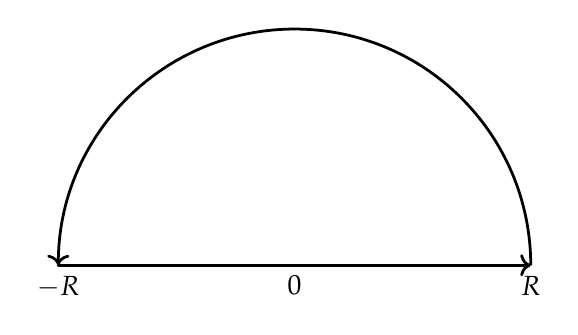
\begin{tikzpicture}[scale=1, transform shape]
    \tkzInit[xmin=-5,ymin=-5,xmax=5,ymax=5]
    \tkzDefPoint(0,0){O}
    \tkzDefPoint(3,0){P}
    \tkzDefPoint(-3,0){Q}
    \tikzset{compass style/.append style={->}}
    \tkzDrawArc[color=black,line width=1pt, ->](O,P)(Q) 
    \tkzDrawSegments[color=black,line width=1pt,->](Q,P)
    \node [below] at (0,0) {$0$};
    \node [below] at (-3,0) {$-R$};
    \node [below] at (3,0) {$R$};
\end{tikzpicture}
\end{center}
\caption{The contour $\gamma_R$}%
\label{fig:}
\end{figure}
then we see that
\[ \int_{\gamma_R} F(z) \dd{z} = \int_{-R}^R F(x) \dd{x} + \int_{\text{arc}} F(z) \dd{z}, \]
and the second term approaches $0$ as $R \to \infty$, so 
\[ \int_{- \infty}^{\infty} F(x) \dd{x} = \lim_{R \to \infty} \int_{\gamma_R} F(z) \dd{z} = 2 \pi i \sum_{\mc{H}} \Res_z f. \]
To see that the integral of the arc disappears, observe that 
\[ \abs{\int_{\text{arc}} F(z) \dd{z}} \leq \pi R \sup_{z \in \text{arc}} \abs{F(z)}. \]
But then if $\deg P = n, \deg Q = m$, $z^{m-n} F(z) \to \frac{a_n}{b_m}$ as $\abs{z} \to \infty$, so we can bound this quantity by some constant $C$, and thus
\[ \abs{\int_{\text{arc}} F(z) \dd{z}} \leq \pi R C \cdot R^{n-m} = \pi C R^{n+1-m} \to 0 \]
as $R \to \infty$ because $n+1-m < 0$.

\begin{exm}
    Consider the integral
    \[ I = \int_{-\infty}^{\infty} \frac{x^2 - x + 2}{x^4 + 10x^2 + 4} \dd{x}. \]
    Then we have simple poles at $z = \pm i, \pm 3i$, so we have
    \begin{align*}
        I &= 2 \pi i \Res_i F + \Res_{3i} F \\
          &= 2 \pi i \qty(\frac{P(i)}{Q'(i)} + \frac{P(3i)}{Q'(3i)}) \\
          &= \frac{5}{12} \pi.
    \end{align*}
\end{exm}

Now consider $F \in \R(x)$ with $\deg P + 1 \leq \deg Q$ and $Q(x) \neq 0$ for $x \in \R$. We want to compute the integral
\[ \int_{- \infty}^{\infty} F(x) e^{ix} \dd{x}. \]
We will consider the contour
\begin{figure}[H]
\begin{center}
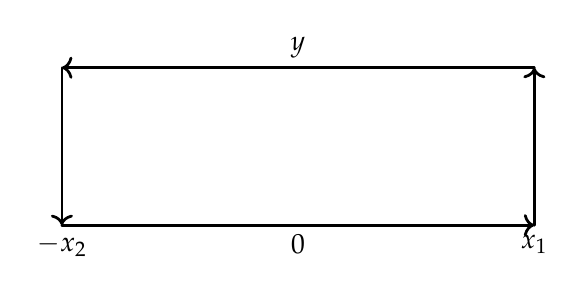
\begin{tikzpicture}[scale=1, transform shape]
    \tkzInit[xmin=-5,ymin=-5,xmax=5,ymax=5]
    \tkzDefPoint(0,0){O}
    \tkzDefPoint(3,0){P}
    \tkzDefPoint(-3,0){Q}
    \tkzDefPoint(-3,2){R}
    \tkzDefPoint(3,2){S}
    \tkzDrawSegments[color=black,line width=1pt,->](Q,P P,S S,R R,Q)
    \node [below] at (0,0) {$0$};
    \node [below] at (-3,0) {$-x_2$};
    \node [below] at (3,0) {$x_1$};
    \node [above] at (0,2) {$y$};
\end{tikzpicture}
\end{center}
\caption{The contour of integration}%
\label{fig:}
\end{figure}

Now we note that 
\[ \abs{\int_{\text{up}}} F(z) e^{iz} \dd{z} \leq y \sup \abs{F(z) e^{iz}} \leq y \sup \abs{F(z)}. \]
Then we know $\abs{F(z)} \leq C \abs{z}^{\deg P - \deg Q}$, so
\[ \abs{\int_{\text{up}} F(z) e^{iz} \dd{z}} \leq \int_0^y \frac{C}{\abs{z}} e^{-y} \dd{y} \leq \int_0^y \frac{C}{x_1} e^{-y} \dd{y} \leq \frac{C}{x_1} \to 0 \]
as $x_1 \to \infty$. By a similar argument, $\int_{\text{down}}$ vanishes in the limit. Finally, we have
\[ \abs{\int_{\text{left}} F(z) e^{iz} \dd{z}} \leq (x_1 + x_2) \frac{C}{y} e^{-y}, \]
and this clearly vanishes in the limit. This gives us
\[ \int_{- \infty}^{\infty} F(x) e^{ix} \dd{x} = 2 \pi i \sum_{{z_j \in \mc{H}}} \Res_{z_j} F(z) e^{iz}. \]
This is because 
\[ \abs{\int_{-x_2}^{x_1} F(x) e^{ix} \dd{x} - 2 \pi i \sum_{z_i \in \mc{H}} \Res_{z_j} F(z)e^{iz}} \leq (x_1 + x_2) \cdot \frac{C}{y}e^{iy} + \frac{C}{x_1} + \frac{C}{x_2}. \]
As $x_1, x_2, y \to \infty$, this vanishes.

\begin{exm}
    Consider the integral $I = \int_{- \infty}^{\infty} \frac{x \sin x}{x^2 + a^2} \dd{x}$ for $a \in \R_{>0}$. We see that $\sin x = \Im(e^{ix})$, so we must have
    \begin{align*}
        I &= \Im\qty(\int_{-\infty}^{\infty} \frac{xe^{ix}}{x^2+a^2} \dd{x}) \\
          &= \Im \qty(2 \pi i \sum_{\mc{H}} \Res \qty(\frac{ze^{iz}}{z^2 + a^2})) \\
          &= \Im\qty(2 \pi i \frac{ia e^{i^2a}}{2ia}) \\
          &= \pi e^{-a}.
    \end{align*}
\end{exm}

Finally, let $\alpha \in [0,1)$ and $F = P/Q$ with $\deg P + 2 \leq \deg Q$ and consider the integral
\[ I = \int_0^{\infty} x^{\alpha} F(x) \dd{x}. \]
Suppose that $Q(x) \neq 0$ for $x \in \R_{>0}$ and at worst has a simple zero at $x = 0$. Then we will consider the contour $\gamma_{r,R, \ep}$, where $r$ is the inner radius, $R$ the outer radius, and $\ep$ the width of the corridor.
\begin{figure}[H]
\begin{center}
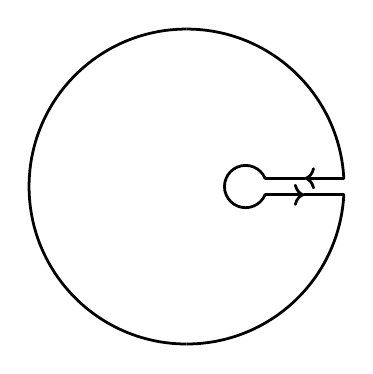
\begin{tikzpicture}[scale=1, transform shape]
    \tkzInit[xmin=-5,ymin=-5,xmax=5,ymax=5]
    \tkzDefPoint(0,0){O}
    \tkzDefPoint(0.75,0){P}
    \tkzDefPoint(3:2){D} \tkzDefPoint(90:2){M} \tkzDefPoint(270:2){N}
    \tkzDefPoint(-3:2){E}
    \tkzDefPoint[shift={(-1,0)}](3:2){B} \tkzDefMidPoint(B,D) \tkzGetPoint{B'}
    \tkzDefPoint[shift={(-1,0)}](-3:2){C} \tkzDefMidPoint(C,E) \tkzGetPoint{C'}
    \tkzDrawArc[color=black,line width=1pt](O,N)(E) 
    \tkzDrawArc[color=black,line width=1pt](P,B)(C)
    \tikzset{compass style/.append style={->}}
    \tkzDrawArc[color=black,line width=1pt](O,D)(M) 
    \tkzDrawArc[color=black,line width=1pt](O,M)(N) 
    \tkzDrawSegments[color=black,line width=1pt,->](D,B' C,C')
    \tkzDrawSegments[color=black,line width=1pt](B',B C',E)
\end{tikzpicture}
\end{center}
\caption{Contour $\gamma_{r,R,\ep}$}%
\label{fig:}
\end{figure}
Now as $\ep \to 0$, we have
\[ \int_{\gamma_{r,R,\ep}} \to \int_{C_R} - \int_{C_r} + \int_{0}^{\infty} x^{\alpha} F(x) \dd{x} - e^{2 \pi i \alpha} \int_0^{\infty} x^{\alpha} F(x) \dd{x}, \]
so we obtain the equation
\[ (1 - e^{2 \pi i \alpha})I + \int_{C_R} - \int_{C_r} = 2 \pi i \sum_p \Res_p z^{\alpha} F(x) \dd{x}. \]
But now we have
\[ \abs{\int_{C_R} z^{\alpha} F(z) \dd{z}} \leq 2 \pi R \sup_{z \in C_R} \abs{z^{\alpha} F(z)} \leq 2 \pi R^{\alpha - 1} \to 0 \]
as $R \to \infty$ because $\abs{z^{\alpha} F} \leq C \cdot R^{\alpha} R^{\deg P - \deg Q} \leq C \cdot R^{\alpha - 2}$. We also have
\[ \abs{\int_{C_r} z^{\alpha} F(z) \dd{z}} \leq 2 \pi r C r^{\alpha - 1} = 2 \pi C r^{\alpha} \to 0 \]
as $r \to 0$ because $\abs{z^{\alpha}F} \leq C r^{\alpha - 1}$. Therefore, we have
\[ (1 - e^{2 \pi i \alpha}) I = 2 \pi i \sum_{p \in \C} \Res_p. \]

\begin{exm}
    Consider the integral $I = \int_0^{\infty} \frac{x^{1/2}}{1 + x^2} \dd{x}$. Then we have
    \begin{align*}
        (1 - e^{\pi i}) I &= 2 \pi i \qty( \Res_i \frac{z^{1/2}}{1+z^2} + \Res_{-i} \frac{z^{1/2}}{1+z^2} ) \\
                          &= 2 \pi i \qty(\frac{e^{\pi/4}}{2i} + \frac{e^{3 \pi/4}}{-2i}) \\
                          &= \pi \sqrt{2}.
    \end{align*}
    Therefore, $I = \frac{\pi}{\sqrt{2}}$.
\end{exm}

\section{Singularities}%
\label{sec:singularities}

We will now consider the next type of singularity. These are the removable singularities.

\begin{thm}[Riemann, removable singularity theorem]
    Let $f \colon \Omega \setminus \qty{z_0} \to \C$ be holomorphic and assume $f$ is bounded on $D \setminus \qty{z_0}$ for some disk $D$ centered at $z_0$. Then $f$ extends to a holomorphic function on $\Omega$ and $z_0$ is a removable singularity.
\end{thm}

\begin{proof}
    Consider the same keyhole as in Figure 2.3 except now with keyholes at $z_0$ and $z$. 
\begin{figure}[H]
\begin{center}
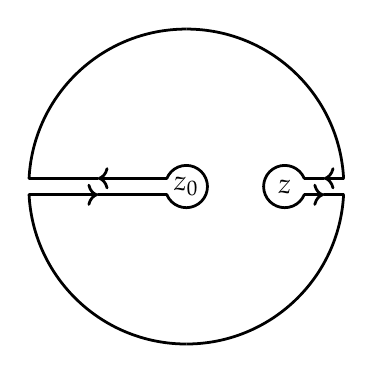
\begin{tikzpicture}[scale=1, transform shape]
    \tkzInit[xmin=-5,ymin=-5,xmax=5,ymax=5]
    \tkzDefPoint(0,0){O}
    \tkzDefPoint(1.25,0){P}
    \tkzDefPoint(3:2){D} \tkzDefPoint(90:2){M} \tkzDefPoint(270:2){N}
    \tkzDefPoint(-3:2){E}
    \tkzDefPoint(177:2){F}
    \tkzDefPoint(183:2){G}
    \tkzDefPoint[shift={(1.75,0)}](177:2){H} \tkzDefMidPoint(H,F) \tkzGetPoint{H'}
    \tkzDefPoint[shift={(1.75,0)}](183:2){I} \tkzDefMidPoint(I,G) \tkzGetPoint{I'}
    \tkzDefPoint[shift={(-0.5,0)}](3:2){B} \tkzDefMidPoint(B,D) \tkzGetPoint{B'}
    \tkzDefPoint[shift={(-0.5,0)}](-3:2){C} \tkzDefMidPoint(C,E) \tkzGetPoint{C'}
    \tkzDrawArc[color=black,line width=1pt](O,N)(E) 
    \tkzDrawArc[color=black,line width=1pt](P,B)(C)
    \tikzset{compass style/.append style={->}}
    \tkzDrawArc[color=black,line width=1pt](O,D)(M) 
    \tkzDrawArc[color=black,line width=1pt](O,M)(F) 
    \tkzDrawArc[color=black,line width=1pt](O,G)(N) 
    \tkzDrawSegments[color=black,line width=1pt,->](D,B' C,C')
    \tkzDrawSegments[color=black,line width=1pt](B',B C',E)
    \tkzDrawSegments[color=black,line width=1pt,->](G,I' H,H')
    \tkzDrawSegments[color=black,line width=1pt](I',I H',F)
    \tkzDrawArc[color=black,line width=1pt](O,I)(H)
    \node at (0,0) {$z_0$};
    \node at (1.25,0) {$z$};
\end{tikzpicture}
\end{center}
\caption{Contour $\gamma$}%
\label{fig:}
\end{figure}
    Then we have
    \[ \int_{\gamma} \frac{f(w)}{w-z} \dd{z} = 0 \]
    by Cauchy's theorem. Therefore, $\int_{\partial D} - \int_{C_1} - \int_{C_2} = 0$, so we see that
    \[ \int_{\partial D} \frac{f(w)}{w-z} \dd{w} = \int_{C_1} \frac{f(w)}{w-z} \dd{w} + \int_{C_2} \frac{f(w)}{w-z} \dd{w}, \]
    where $C_1$ is a circle centered at $z_0$ and $C_2$ is a circle centered at $z$. Then as $r \to 0$, we see that $\int_{C_1} \to 0$. But now we can set $f(z) \coloneqq \frac{1}{2 \pi i} \int_{\partial D} \frac{f(w)}{w-z} \dd{w}$, so $f$ is holomorphic at $z$.
\end{proof}

\begin{cor}
    Let $f \colon \Omega \setminus \qty{z_0} \to \C$ be holomorphic. Then $f$ has a pole at $z_0$ if and only if $f(z) \to \infty$ as $z \to z_0$.
\end{cor}

\begin{proof}
    We know that $f$ has a pole if and only if 
    \[ g = \begin{cases}
        \frac{1}{f} & z \neq z_0 \\
        0 & z = z_0
    \end{cases} \]
    is holomorphic near $z_0$. Therefore $f$ has a pole if and only if $\frac{1}{f} \to 0$ as $z \to z_0$, which is equivalent to $f(z) \to \infty$.
\end{proof}

Now we will consider the final type of singularity: \textit{essential singularities}. This is every singularity that is not a pole or a removable singularity. The canonical example is $f(z) = e^{1/z} \colon \C \setminus \qty{0} \to \C$.

\begin{thm}[Casorati-Weierstrass]
    Let $f \colon \Omega \setminus \qty{z_0} \to \C$ be holomorphic and $z_0$ be an essential singularity. Then $f(\Omega \setminus \qty{z_0})$ is dense in $\C$. Equivalently, for all $\alpha \in \C$, there exists $z_n \in \Omega \setminus \qty{z_0}$ such that $z_n \to z_0$ and $f(z_n) \to \alpha$.
\end{thm}

\begin{proof}
    Assume there exists $\alpha \in \C$ such that $\abs{f(z) - \alpha} > \delta$ for all $z \in \Omega$ and some $\delta > 0$. Then if we write $g(z) = \frac{1}{f(z) - \alpha}$, we see that $\abs{g(z)} < \delta^{-1}$, so $g$ is holomorphic on $\Omega$. Therefore, we have $f(z) = \frac{1}{g(z)} + \alpha$. If $g(z_0) \neq 0$, then $f$ has a removable singularity, and if $g(z_0) = 0$, then $f$ has a pole.
\end{proof}

Finally, we will consider Laurent series expansions.

\begin{prop}
    Let $f \colon \Omega \to \C$ be holomorphic and $A = \qty{z \mid r_1 < \abs{z-z_0} < r_2}$ and assume $\abs{A} \subset \Omega$. Then $f(z) = \sum_{n = -\infty}^{\infty} a_n {(z-z_0)}^n$ for all $z \in A$.
\end{prop}

\begin{proof}
    Consider the keyhole
    \begin{figure}[H]
    \begin{center}
    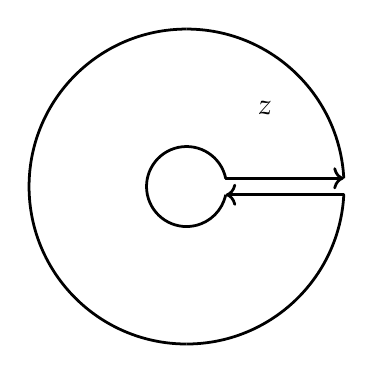
\begin{tikzpicture}[scale=1, transform shape]
        \tkzInit[xmin=-5,ymin=-5,xmax=5,ymax=5]
        \tkzDefPoint(0,0){O}
        \tkzDefPoint(3:2){D} \tkzDefPoint(90:2){M} \tkzDefPoint(270:2){N}
        \tkzDefPoint(-3:2){E}
        \tkzDefPoint[shift={(-1.5,0)}](3:2){B} \tkzDefMidPoint(B,D) \tkzGetPoint{B'}
        \tkzDefPoint[shift={(-1.5,0)}](-3:2){C} \tkzDefMidPoint(C,E) \tkzGetPoint{C'}
        \tkzDrawArc[color=black,line width=1pt](O,N)(E) 
        \tkzDrawArc[color=black,line width=1pt](O,B)(C)
        \tikzset{compass style/.append style={->}}
        \tkzDrawArc[color=black,line width=1pt](O,D)(M) 
        \tkzDrawArc[color=black,line width=1pt](O,M)(N) 
        \tkzDrawSegments[color=black,line width=1pt,<-](D,B' C,C')
        \tkzDrawSegments[color=black,line width=1pt](B',B C',E)
        \node at (1,1) {$z$};
    \end{tikzpicture}
    \end{center}
    \caption{Contour $\gamma_{\ep}$}%
    \label{fig:}
    \end{figure}
    Now note that $f(z) = \frac{1}{2 \pi i} \int_{\gamma_{\ep}} \frac{f(w)}{w-z} \dd{w}$, so as $\ep \to 0$, we see that $\int_{\gamma_{\ep}} \to \int_{C_{r_2}} - \int_{C_{r_1}}$. Now we obtain
    \begin{align*}
        \int_{C_{r_2}} \frac{f(w)}{w-z} \dd{w} &= \int_{C_{r_2}} \frac{f(w)}{(w-z_0) - (z-z_0)} \dd{w} \\
                                               &= \int_{C_{r_2}} \frac{1}{w-z_0} \frac{f(w)}{1 - \frac{z-z_0}{w-w_0}} \\
                                               &= \int_{C_{r_2}} \frac{1}{w-z_0} f(w) \sum_{n=0}^{\infty} {\qty(\frac{z-z_0}{w-w_0})}^n \dd{w} \\
                                               &= \sum_{n=0}^{\infty} \qty(\int_{C_{r_2}} \frac{1}{{(w-z_0)}^{n+1}} f(w) \dd{w}) \cdot {(z-z_0)}^n.
    \end{align*}
    Similarly, we have 
    \begin{align*}
        \int_{C_{r_1}} \frac{f(w)}{w-z} \dd{w} &= \int_{C_{r_1}} \frac{1}{z-z_0} \frac{f(w)}{\frac{w-z_0}{z-z_0}-1} \dd{w} \\
                                               &= \int_{C_{r_1}} \frac{1}{z-z_0} (-f(w)) \sum_{n=0}^{\infty} {\qty(\frac{w-z_0}{z-z_0})}^n \dd{w} \\
                                               &= \sum_{n=0}^{\infty} \int_{C_{r_1}} -f(w) {(w-z_0)}^n {(z-z_0)}^{-(n+1)}.
    \end{align*}
    Combining, we obtain the desired result.
\end{proof}

In the special case where $r_1 = 0$, then if $f \colon \Omega \setminus \qty{z_0} \to \C$ is holomorphic with $D \subset \Omega$, then we can write
\[ f(z) = \sum_{n=-\infty}^{\infty} a_n {(z-z_0)}^n \]
on $D \setminus \qty{z_0}$. Therefore the types of singularities correspond to
\begin{description}
    \item[Removable:] For all $n < 0$, $a_n = 0$.
    \item[Pole:] There exists $k > 0$ such that $a_n = 0$ for all $n < -k$.
    \item[Essential:] For all $N > 0$, there exists $n > N$ such that $a_{-n} \neq 0$.
\end{description}
Now we see that $e^{1/z} = \sum_{n=0}^{\infty} \frac{z^{-n}}{n!}$ has an essential singularity at $0$.

\begin{rmk}
    The Laurent series expansion is unique.
\end{rmk}

\begin{warn}
    We \textbf{cannot} write $a_n = \frac{f^{(n)}(z_0)}{n!}$.
\end{warn}

\section{Meromorphic Functions}%
\label{sec:meromorphic_functions}

First, we will define the Riemann sphere $\P^1 = \C\P^1 = \C \cup \qty{\infty}$. Here, we consider stereographic projection $S^2 \setminus \qty{(0,0,1)} \to \C$. This is given by the formula $\varphi(x,y,z) = \frac{1}{1-z} (x+iy)$. This gives us a homeomorphism $S^2 \to \C\P^1$, and the topology on $\C\P^1$ is induced by this identification. This is a special case of the one-point compactification. In fact, we will see that $\C\P^1$ has more structure: that of a \textit{Riemann surface}, or a $1$-dimensional complex manifold.

\begin{defn}
    A \textit{Riemann surface} $X$ is a topological space $X$ with an atlas of charts $X = \bigcup_{\alpha} U_{\alpha}$ with homeomorphisms $\varphi_{\alpha} \colon U_{\alpha} \to V_{\alpha} \subseteq \C$ such that the transition maps 
    \[ \varphi_{\beta} \circ \varphi_{\alpha}^{-1} \colon \varphi_{\alpha}(U_{\alpha} \cap U_{\beta}) \to \varphi_{\beta}(U_{\alpha} \cap U_{\beta}) \] 
    are holomorphic. We also require that $X$ is connected, Hausdorff, and second-countable.
\end{defn}

\begin{exm}
    On $\C\P^1$ we may consider the two charts $S^2 = U_1 \cup U_2$ with the two charts given by $\varphi_1$ being stereographic projection and $\varphi_2$ being stereographic projection from the south pole followed by conjugation. We can check that the transition map
    \[ \varphi_2 \circ \varphi_1^{-1} \qty(\frac{x+iy}{1-z}) = \frac{x-iy}{1+z} = {\qty(\frac{x+iy}{1-z})}^{-1}, \]
    so $\varphi_2 \circ \varphi_{-1} (w) = \frac{1}{w}$. Therefore $\P^1$ can be given the structure of a \textbf{compact} Riemann surface with two charts $U_1 = \C \xrightarrow{\mr{id}} \C$ and $U_2 = \C \cup \infty \setminus 0 \xrightarrow{z \mapsto 1/z} \C$.
\end{exm}

\begin{exm}
    The second example of a Riemann surface is an elliptic curve. Choose $\lambda_1, \lambda_2 \in \C$ linearly independent over $\R$. Then if we write $\Lambda = \Z \lambda_1 + \Z \lambda_2$, we can set $X = \C/\Lambda$. This has the quotient topology from $\C$. To define charts, let $U_{z_0}$ be a small disk in $\C$ centered at $z_0$. Then under the map $q \colon \C \to X$, we have a homeomorphism $D \to q(D)$ and transition functions are given by $z \mapsto z + \lambda$ for some $\lambda \in \Lambda$.
\end{exm}

\begin{rmk}
    It is also possible to define Riemann surfaces without using topology. We simply define the $U_{\alpha}$ as \textbf{sets} with bijections to open subsets of $\C$ and then specify holomorphic transition maps. Then the topology is given by the topology from $\C$, where each $U_{\alpha}$ is open. This allows for non-Hausdorff examples, like two copies of $\C$ glued by the identity map on $\C \setminus \qty{0}$, called the \textit{affine line with two origins}.\footnote{This can be given a natural structure as a scheme. For more information about this, read a book about algebraic geometry.} 
\end{rmk}

\begin{rmk}
    If $X, Y$ are Riemann surfaces, we can define holomorphic maps $F \colon X \to Y$. If we choose charts $p \in U \xrightarrow{\varphi} \C$ and $F(p) \in V \xrightarrow{\psi} \C$, then we require that $\psi F \varphi^{-1}$ is holomophic and that $F$ is continuous.
\end{rmk}

Now the definition of a pole is equivalent to the map $\wt{f} \colon \Omega \to \P^1$ given by $\wt{f}(z) = f(z)$ when $z \neq z_0$ and $f(z_0) = \infty$ being holomorphic. Similarly, being meromorphic is equivalent to being a holomorphic map to $\C\P^{\infty}$. 

\begin{defn}
    Let $f \colon \Omega \to \C$ be holomorphic and suppose there exists $R > 0$ such that $\qty{z \mid \abs{z} > R} \subset \Omega$. Then we can define $g \colon \qty{x \mid 0 < \abs{z} < \frac{1}{R}} \to \C$ by $g(z) = f(1/z)$. Then we say that $f$ has a (removable singularity, pole of order $k$, essential singularity) at $\infty$ if $g$ has the same thing at $z = 0$.
\end{defn}

\begin{exm}
    If $f = \frac{P}{Q}$ is a rational function and $\deg P = n, \deg Q = m$, then $f$ has a removable singularity at $\infty$ if $m \geq n$ and a pole of order $n-m$ if $m < n$. In particular, $f$ is meromorphic on $\C \cup \infty$.
\end{exm}

\begin{exm}
    We know that $f(z) = e^{z}$ has an essential singularity at $\infty$ because $g(z) = e^{z^{-1}}$ has an essential singularity at $0$.
\end{exm}

\begin{thm}
    The meromorphic functions on $\P^1$ are the rational functions.
\end{thm}

\begin{proof}
    Let $f \colon \P^1 \to \P^1$ be meromorphic. Note that the number of poles is finite because $\P^1 = S^2$ is compact. Then let the poles be $z_1, \ldots, z_n$ and possibly $\infty$. Then at $z_i$, we expand $f$ as a Laurent series and write
    \[ f_i(z) = \sum_{j=1}^{m_i} a_{ij} {(z-z_i)}^{-j} + g_i(z), \]
    where $g_i$ is holomorphic near $z_i$. By construction, $g = f - \sum_{i=1}^n f_i$ is holomorphic on $\C$. Now consider $h(z) = g(z^{-1})$ near $z = 0$. We have 
    \[ h(z) = \sum_{j=1}^{m_{\infty}} a_{\infty j} z^{-j} + g_{\infty}(z), \]
    so 
    \[g(z) = h(z^{-1}) = \sum_{j=1}^{m_{\infty}} a_{\infty j} z^j + g_{\infty}(z^{-1}). \]
    Therefore If we write the first term as a polynomial $p(z)$, $g_{\infty}(z^{-1})$ is bounded as $z \to \infty$, so by Liouville it is constant. Finally, we have $f = c + p(z) + \sum f_i(z)$, which is rational.
\end{proof}

\begin{rmk}
    Let $f = \frac{p}{q}$ be rational and suppose $p,q$ are coprime and nonconstant. Then the number of zeros of $f$ is equial to the number of poles of $f$, and both are given by $\max (\deg p, \deg q)$. This follows from the fundamental theorem of algebra and the calculuation of the behavior of $f$ at $\infty$.
\end{rmk}

More generally, if $f \colon X \to Y$ is a nonconstant holomorphic map between compact Riemann surfaces, we can define a well-defined \textit{degree} of $f$ by $\abs{f^{-1}(q)} = \deg f$ counting multiplicity. We can now consider the automorphisms of $\P^1$. Clearly these are rational maps, and the maps given by
\[ f(z) = \frac{az + b}{cz + d} \qquad a,b,c,d \in \C, ad-bc \neq 0 \]
have inverse $w \mapsto \frac{dz - b}{-cw + a}$. In fact, these are actually all automorphisms because any automorphism $f = \frac{p}{q}$ must satisfy $\deg f = \max (\deg p, \deg q) = 1$. Also, for all but finitely many $c \in \C$, all solutions of $f(z) = c$ have multiplicity $1$. Therefore, we have $\Aut(\P^1) = PGL_2(\C)$ because we can identify $\P^1 = \C^2 \setminus \qty{0} / \C^{\times}$ and then the point $(z_1 : z_2)$ corresponds to $\frac{z_1}{z_2}$. Then it is easy to see that these fractional linear transformations correspond to matrix multiplication.

With the prior discussion, we may now use the residue theorem at $\infty$.
\begin{exm}[Fall 2016 Qualifying Exam, Q9]
    Consider $C = \qty{z \in \C \mid \abs{z} = 2}$ oriented counterclockwise and let $n \in \Z$ satisfy $n \geq 2$. We want to compute
    \[ I = \int_C \frac{z^{2n} \cos(1/z)}{1-z^n}. \]
    Note that the residue theorem applies to essential singularities, so we may set $w = \frac{1}{z}, \dd{z} = \frac{-1}{w^2} \dd{w}$. Therefore we have
    \[ I = - \int_{C_{1/2}} \frac{\cos w}{w^{n+2}(w^n - 1)} = 2 \pi i \Res_0 \frac{\cos w}{w^{n+2}(w^n - 1)} = \begin{cases}
        \frac{{(-1)}^{\frac{n+3}{2}}}{(n+1)!} & n \text{ odd} \\
        0 & \text{otherwise}.
    \end{cases} \]
\end{exm}

\section{Estimates for Holomorphic Functions}%
\label{sec:estimates_for_holomorphic_functions}

\begin{thm}[Argument principle]
    Let $f$ be meromorphic on $\Omega \subset \C$ and $\gamma$ be a simple closed curve such that $\gamma$ and its interior are contained in $\Omega$. Suppose $f$ is holomorphic and nonzero on $\gamma$, oriented positively. Then
    \[ \frac{1}{2 \pi i} \int_{\gamma} \frac{f'(z)}{f(z)} \dd{z} = \#\qty{\text{zeroes of $f$ inside $\gamma$}} - \#\qty{\text{poles of $f$ inside $\gamma$}}. \]
\end{thm}

\begin{proof}
    Use the residue theorem. We have
    \[ \frac{1}{2 \pi i} \int_{\gamma} \frac{f'(z)}{f(z)} \dd{z} = \sum_{z_0} \Res_{z_0} \frac{f'}{f}. \]
    But then if $z_0$ is a zero or pole of order $n$, we have
    \[ \Res_{z_0} \frac{f'}{f} = \Res_{z_0} \qty(\frac{n{(z-z_0)}^{n-1}}{{(z-z_0)}^n}) = n. \]
\end{proof}

\begin{rmks}
    The left hand-side of the formula is the winding number of $f \circ \gamma$ around $z = 0$. In addition, we can think of $\frac{f'}{f} \dd{z}$ as $\dd{(\log f)}$, but $\log z$ is not well-defined.
\end{rmks}

\begin{thm}[Rouch\'e]
    Let $f, g \colon \Omega \to \C$ be holomorphic and $\gamma$ be a simple closed curve with $\gamma + \mr{int}(\gamma) \subset \Omega$. Assume that $\abs{f(z)} > \abs{g(z)}$ for all $z \in \gamma$. Then the number of zeroes of $f$ inside $\gamma$ is equal to the number of zeroes of $f + g$ inside $\gamma$, counting multiplicity.
\end{thm}

\begin{proof}
    Define for $t \in [0,1]$ the function $f_t = f + tg \colon \Omega \to \C$. This is holomorphic on $\Omega$ and nonzero on $\gamma$. Then the function
    \[ n(t) \coloneqq \frac{1}{2 \pi i} \int_{\gamma} \frac{f_t'(z)}{f_t(z)} \dd{z} \in \Z \]
    is continuous because the integrand depends continuously on $t$, but $\Z$ is discrete, so it must be constant.
\end{proof}

\begin{exm}
    Consider $f = z^5$, $g = 3z + 1$. Then if $\abs{z} = 2$, $\abs{f(z)} = 32$ while $\abs{g(z)} \leq 3 \cdot 2 + 1 = 7$, so $f + g$ has $5$ zeroes with $\abs{z} < 2$. On the other hand, if $\abs{z} = 1$, then $\abs{g} \geq 2$ while $\abs{f} = 1$, so $f + g$ has a single zero with $\abs{z} < 1$.
\end{exm}

\begin{thm}[Open mapping theorem]
    Let $f \colon \Omega \to \C$ be holomorphic and nonconstant on a connected $\Omega$. If $U \subset \Omega$ is open, then $f(U)$ is open.
\end{thm}

\begin{proof}
    Let $z_0 \in \Omega$ and write $w_0 = f(z_0)$. We need to show that for some $\ep > 0$, the set
    \[ \qty{w \mid \abs{w-w_0} < \ep} \subset f(\Omega). \]
    Equivalently, we want to show that $f(z) - w = 0$ has a solution $z \in \Omega$ for $\abs{w-w_0} < \ep$. Choose $\delta > 0$ such that $\ol{D} = \qty{z \mid \abs{z-z_0} \leq \delta} \subset \Omega$. For $\delta$ small enough, $f(z) \neq w_0$ for $\abs{z-z_0} = \delta$. Then we know $\abs{f(z) - w_0} > \ep$ on $\partial D$ for some $\ep > 0$, so for $\abs{w-w_0} < \ep$, Rouche's theorem tells us that the number of zeroes of $(f(z) - w_0) + (w_0 - w)$ is equal to the number of zeroes of $f(z) - w_0$ in $D$, and this is positive.
\end{proof}

\begin{thm}[Maximum Principle]
    Let $f \colon \Omega \to \C$ be holomorphic on some open set $\Omega \subset \C$. Then $\abs{f}$ does \textbf{not} attan a maximum on $\Omega$.
\end{thm}

\begin{proof}
    Given $z_0 \in \Omega$, we know $f(z_0) \in \qty{w \mid \abs{w - f(z_0)} < \ep} \subset f(\Omega) \subset \C$. Clearly there exists $w \in D$ such that $\abs{w} > \abs{f(z_0)}$.
\end{proof}

Here is another formulation. Suppose $f \colon \Omega \to \C$ is holomorphic and $f$ extends continuously to $\ol{\Omega}$, which is bounded. Then the maximum of $f$ on $\ol{\Omega}$ is obtained on the boundary, so we cannot obtain the maximum on $\Omega$.

\begin{rmk}
    Suppose $f \colon \Omega \to \C$ is holomorphic and nonconstant on a connected $\Omega$. Then the real part of $f$ does not attain a maximum on $\Omega$. Here, we simply apply the maximum principle to $g = e^f$.
\end{rmk}

Now recall that if $f = u + iv$ and $f$ is holomorphic, then $u, v$ are harmonic. This means that $\pdv[2]{u}{x} + \pdv[2]{u}{y} = 0$. Conversely, if $u$ is a harmonic funciton on a disk $D \subset \C = \R^2$, there exists a harmonic $v$ such that $f = u+iv$ is holomorphic on $D$. Therefore we obtain a maximum principle for harmonic functions. The physical intuition for this is that if $u \colon \ol{\Omega} \to \R$ is harmonic and we fix $\eval{u}_{\partial \Omega}$, then this corresponds to the steady state temperature of points in the region $\Omega$. Then heat would flow away from a maximum, so the maximum cannot be attained on the interior.

Now recall from multivariable calculus that if $f \colon \R^2 \to \R$, we have critical points of $f$ when 
\[ \eval{ \pdv{f}{x} }_p = \eval{\pdv{f}{y}}_p = 0. \]
Then we may consider the matrix
\[ \mqty( \pdv[2]{f}{x} & \pdv{f}{y}{x} \\ \pdv{f}{x}{y} & \pdv[2]{f}{y} ) \eqqcolon H. \]
This is called the \textit{Hessian} of $f$. If we assume that $p = (0,0)$, then we can write
\[ f(x,y) = f(0,0) + \pdv[2]{f}{x}(0,0) x^2 + 2 \pdv{f}{x}{y} (0,0) xy + \pdv[2]{y}(0,0) y^2 + O(\norm{x,y}^3). \]
If $\det H \neq 0$, then we have a nondegenerate quadratic form. After a linear change of coordinates, theere are three cases:
\begin{enumerate}
    \item The form looks like $x^2 + y^2$ and $\det H > 0$. This is a minimum.
    \item The form looks like $-(x^2 + y^2)$ and $\det G > 0$. This is a maximum.
    \item The form looks like $x^2 - y^2$ and $\det H < 0$. This is a saddle point.
\end{enumerate}
For any harmonic function, any nondegenerate critical point is a saddle point because
\[ \det H = - {\qty(\pdv[2]{u}{x})}^2 - {\qty(\pdv{u}{x}{y})}^2 \leq 0. \]
\begin{exm}
    Consider $f(z) = z^2$. Then $u = x^2 - y^2 = (x+y)(x-y)$ and $v = 2xy$. Clearly the origin is a saddle point for both. The graph of $u$ looks like
    \begin{figure}[H]
    \begin{center}
    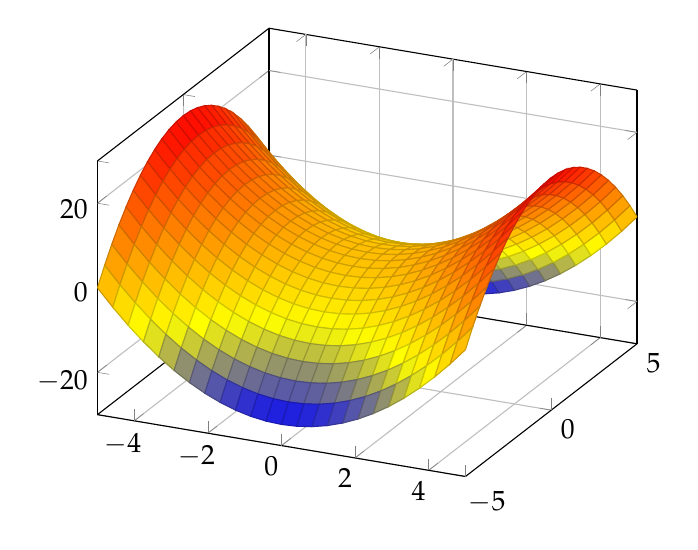
\begin{tikzpicture}[scale=1, transform shape]
        \begin{axis}[grid=both]
            \addplot3 [surf] {(x^2 - y^2)};
        \end{axis}
    \end{tikzpicture}
    \end{center}
    \caption{Graph of $z = x^2 - y^2$}%
    \label{fig:}
    \end{figure}
\end{exm}

\begin{exm}
    Consider $f(z) = z^3$. Then $u = x^3 - 3xy^2 = x(x-\sqrt{3}y)(x+\sqrt{3}y)$ is not nondegenerate at the origin. The graph looks like
    \begin{figure}[H]
    \begin{center}
    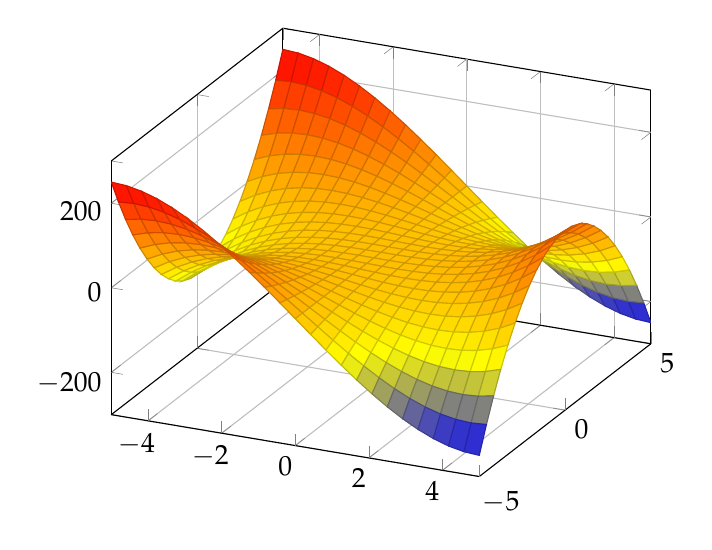
\begin{tikzpicture}[scale=1, transform shape]
        \begin{axis}[grid=both]
            \addplot3 [surf] {(x^3 - 3*x*y^2)};
        \end{axis}
    \end{tikzpicture}
    \end{center}
    \caption{Graph of $z = x^3 - 3xy^2$}%
    \label{fig:}
    \end{figure}
\end{exm}

Now we can give another proof of the maximum principle using the mean-value property. Recall that 
\[ f(z_0) = \frac{1}{2 \pi i} \int_{\gamma} \frac{f(w)}{w-z_0} \dd{w}. \]
Now we parameterize $\gamma$ by $w = z_0 + re^{i \theta}$, so we obtain
\[ f(z_0) = \frac{1}{2 \pi i} \int_0^{2 \pi} \frac{f(z_0 + re^{i\theta})}{re^{i\theta}} ire^{i\theta} \dd{\theta} = \frac{1}{2\pi} \int_0^{2 \pi} f(z_0 + re^{i\theta}) \dd{\theta}, \]
and therefore $f(z_0)$ is the mean value of $f$ on the circle $\gamma$. Therefore, if $f$ is nonconstant, it obtains some larger value on the circle $\gamma$.

\section{The Logarithm}%
\label{sec:the_logarithm}

Let $\Omega \subset \C$ and $\gamma_0, \gamma_1$ be two curves in $\Omega$ with the same endpoints $\alpha, \beta$ and parameterizations $z_0, z_1 \colon [a,b] \to \Omega$. Then $\gamma_0, \gamma_1$ are \textit{homotopic} in $\Omega$ if there exists a continuous 
\[ F \colon [a,b] \times [0,1] \to \Omega \qquad F(s,0) = z_0(s), F(s,1) = z_1(s), F(a,t) = \alpha, F(b,t) = \beta. \]

\begin{thm}
    Let $f$ be holomorphic on $\Omega$ and $\gamma_0, \gamma_1$ curves in $\Omega$. If $\gamma_0, \gamma_1$ are homotopic, then
    \[ \int_{\gamma_0} f(z) \dd{z} = \int_{\gamma_1} f(z) \dd{z}. \]
\end{thm}

\begin{proof}
    Choose a homotopy $F$. Then the image $K$ of $F$ is compact and $K \subset \Omega \subset \C$, so there exists $\ep > 0$ such that for all $w \in K$ the disk $D(z, \ep) \subset \Omega$. We need to show that the distance $d(p,q), p \in K, q \in \C \setminus \Omega$ is bounded below by $\ep > 0$. Otherwise, there exists $p_n \in K$ and $q_n \in \C$ such that $d(p_n, q_n) \to 0$. But then $K$ is compact, so $p_n \to p \in K$, so $q_n \to p$ as well. But then $\C \setminus \Omega$ is closed, and thus $p \in \C \setminus \Omega$, which is a contradiction.

    $F$ is uniformly continuous, so given $\ep > 0$, there exists $\delta > 0$ such that $\abs{F(s_1,t_1) - F(s_2, t_2)} < \ep$ whenever $\abs{(s_1,t_1) - (s_2,t_2)} < \delta$. If we fix $t_1, t_2$ such that $\abs{t_1 - t_2} < \frac{1}{2} \delta$, then we can choose a subdivision $a = s_0 < s_1 < \cdots < s_n = b$, where $s_{i+1} - s_i < \frac{\delta}{2}$. Then we see that $\abs{z_t(s) - z_{t'(s')}} < \ep$ for all $(s,t), (s',t') \in [s_i, s_{i+1}] \times [t_1, t_2]$. But now we choose $D$ to be a disk of radius $\ep$ such that $F([s_i, s_{i+1}] \times [t_1, t_2]) \subset D$. By the Cauchy formula for the disk, we see that
    \[ \int_{\text{perimeter}} f(z) \dd{z} = 0. \]
    Summing over $i$, we see that $\int_{\gamma_{t_1}} - \int_{\gamma_{t_2}} = 0$. Subdividing in the $t$ direction, we get $\int_{\gamma_0} = \int_{\gamma_1}$.
\end{proof}

Now let $\Omega \subset \C$ be open. We sau that $\Omega$ is \textit{simply connected} if it is path connected and any two paths with the same endpoints are homotopic. Equivalently, $\Omega$ is path-connected and any loop $\gamma$ is homotopic to the constant loop.

\begin{exm}
    Any convex set is homotopic by the straight line homotopy
    \[ z_t(s) = (1-t) z_0(s) + t z_1(s) \colon z_0 \Rightarrow z_1. \]
\end{exm}

\begin{exm}
    The set $\C \setminus (-\infty, 0]$ is simply connected. Note that this set is homeomorphic to $\R_{> 0} \times (-\pi, \pi)$ because any $z \in \Omega$ can be uniquely written as $z = re^{i\theta}$ for any $r > 0$ and $\theta \in (-\pi, \pi)$. Therefore, $\Omega$ is homeomorphic to a convex set and is thus simply connected.
\end{exm}

\begin{thm}
    Let $\Omega \subset \C$ be open and connected. Then $\Omega$ is simply connected if and only if $\P^1 \setminus \Omega$ is connected.
\end{thm}

\begin{exm}
    Consider $\R \times (0,1)$. Then the complement in $\P^1$ is connected because $\infty$ joins the two components of $\C \setminus (\R \times (0,1))$.
\end{exm}

\begin{thm}
    Let $\Omega \subset \C$ be simply connected and $f \colon \Omega \to \C$ be holomorphic. Then $f$ has a primitive.
\end{thm}

\begin{proof}
    Fix a basepoint $z_0 \in \Omega$. Then set $F(z) \coloneqq \int_{\gamma_z} f(w) \dd{w}$, where $\gamma_z$ is a path from $z_0$ to $z$ in $\Omega$. Because $\Omega$ is simply-connected, this is well-defined. Now as in the case of the disk, we see that $F'(z) = f(z)$.
\end{proof}

\begin{exm}
    Consider $\Omega = \C \setminus \qty{0}$ and $f(z) = \frac{1}{z}$. Then we see that 
    \[ \int_{S^1} \frac{1}{z} \dd{z} = 2 \pi i \neq 0, \]
    and therefore $\frac{1}{z}$ does not have a primitive, so $\Omega$ is not simply-connected.
\end{exm}

Now we may define the complex logarithm.

\begin{thm}
    Let $\Omega \in \C$ be simply connected with $1 \in \Omega$ and $0 \notin \Omega$. Then there exists a unique holomorphic function $F = \log_{\Omega} \colon \Omega \to \C$ such that $e^{F(z)} = z$ for all $z \in \Omega$ and $F(1) = 0$.
\end{thm}

\begin{proof}
    Let $F$ be a primitive of $\frac{1}{z}$ on $\Omega$ normalized such that $F(1) = 0$. Then we show that $e^{F(z)} = z$. Here, we have
    \[ \dv{z}(ze^{-F(z)}) = e^{-F(z)} + z(-F'(z)) e^{-F(z)} = 0, \]
    so $ze^{-F(z)} = c$ for some constant $c \in \C$. Setting $z = 1$, we obtain $c = 1$, so $e^{F(z)} = z$.

    Now we consider uniqueness of the logarithm. Let $G$ be another such function. Then $G - F \colon \Omega \to 2 \pi i \Z$, but $\Omega$ is connected, so $G-F$ is constant and thus evaluating at $z = 1$ gives us $G = F$.
\end{proof}

\begin{exm}
    Consider $\Omega = \C \setminus (-\infty, 0]$. Then we defined earlier that for $z = re^{i\theta}$, $\log z = \log r + i \theta$.
\end{exm}

More generally, we have the following result.
\begin{thm}
    Let $\Omega \subset \C$ be simply connected and $f \colon \Omega \to \C$ be holomorphic and nowhere vanishing. Then there exists $g \colon \Omega \to \C$ such that $e^g = f$.
\end{thm}

\begin{proof}
    Let $g$ be a primitive of $\frac{f'}{f}$. Then we have
    \[ \dv{z} (f \cdot e^g) = f' e^{-g} - f g' e^{-g} = 0, \]
    so we can simply adjust $g$ by a constant until $fe^{-g} = 1$.
\end{proof}

Now we may define $f^{\alpha} = e^{\alpha \log f}$ for any $\alpha \in \C$.

\chapter{Global Theory}%
\label{cha:global_theory}

\section{Conformal Mappings}%
\label{sec:conformal_mappings}

\begin{quest}
    Let $\Omega_1, \Omega_2 \subset \C$ be open. Does there exist a holomorphic bijection $\Omega_1 \to \Omega_2$?
\end{quest}

\begin{rmk}
    A holomorphic bijection has holomorphic inverse.
\end{rmk}

Our goal will be to prove the following remarkable theorem.
\begin{thm}[Riemann Mapping Theorem]\label{thm:rmt}
    Let $\Omega \subset \C$ be open. Then there exists a holomorphic bijection $F \colon \Omega \to D$ if and only if $\Omega$ is simply connected and $\Omega \neq \C$. Here, $D$ is the unit disk.
\end{thm}

\begin{exm}
    Let $\Omega = \mc{H} = \qty{z = x + iy \mid y > 0} \subset \C$. Then there exists a holomorphic bijection $F \colon \mc{H} \to D$. Note that if $z \in \mc{H}$, then $\abs{z-i} < \abs{z + i}$. Therefore, we can set $F(z) = \frac{i-z}{i+z}$. To see that this is a bijection, we note that $\infty \mapsto -1$, $-i \mapsto \infty$. Therefore, $F \colon \C \setminus \qty{-i} \to \C \setminus \qty{-1}$ is a bijection, and thus it restricts to a bijection $\mc{H} \to D$ on the northern hemisphere.
\end{exm}

\begin{rmk}
    Consider the map $\varphi \colon S^2 \to \P^1$. Then 
    \[ \varphi^{-1}(D) = \qty{(x,y,z) \in S^2 \mid z < 0} \qquad \varphi^{-1} (\mc{H}) = \qty{(x,y,z) \in S^2 \mid y > 0}. \]
    Then if $r$ is the rotation by $\frac{\pi}{2}$ about the $x$-axis, the diagram
    \begin{equation*}
    \begin{tikzcd}
        \qty{z < 0} \ar{r}{r}[swap]{\sim} \ar{d}{\varphi}[swap]{\sim} & \qty{y > 0} \ar{d}{\varphi}[swap]{\sim} \\
        D \ar{r}{\wt{G}} & \mc{H}
    \end{tikzcd}
    \end{equation*}
    commutes, where $\wt{G} = F^{-1} \circ \psi$, where $\psi(w) = iw$.
\end{rmk}

Here, rotation of $S^2$ corresponds to a holomorphic automorphism of $\P^1$ under $\varphi$. This is because stereographic projection preserves angles and rotations also preserve angles. Therefore $\wt{G} = \varphi \circ r \circ \varphi^{-1}$ will preserve angles, so it is holomorphic. This gives us a homomorphism $SO(3) \hookrightarrow \Aut(\P^1) = PGL_2(\C)$. Recall that
\[ SO(3) = \qty{A \in GL_3(\R) \mid A^T A = I, \det A = 1}, \]
The image of the homomorphism is $PSU(2)$, where we have
\[ SU(2) = \qty{B \in GL_2(\C) \mid \ol{B}^T B = I, \det B = 1}. \]
In fact, any $B \in SU(2)$ has the form $B = \begin{psmallmatrix}
    a & b \\
    -\ol{b} & \ol{a}
\end{psmallmatrix}$, so $SU(2) \simeq S^3$. Then we have $PSU(2) = SU(2) / \pm I$. Now we have a chain of isomorphisms
\[ \R\P^3 = S^3 / \pm 1 \cong SO(3) \xrightarrow{\sim} PSU(2) \xleftarrow{2:1} SU(2) \cong S^3, \]
and this is somehow related to the spin of an electron.

Now here are some examples of conformal maps:
\begin{enumerate}
    \item If $f \colon \C \to \C$ is a holomorphic bijection, then there exists $x,y$ such that $f(z) = az + b$.
    \item Let $n \in \N$ and set $S = \qty{z \in \C \mid 0 < \arg(z) < \frac{\pi}{n}}$. Then $z \mapsto z^{\alpha}$ gives a holomorphic bijection $S \to \mc{H}$. If $\alpha > \frac{1}{2}$ is real, then we may consider $z \mapsto z^{\alpha}$.
    \item Consider $\log z = \log r + i \theta$. This gives a holomorphic bijection $\C \setminus (-\infty, 0] \to \R \times i (-\pi, \pi)$. Restricting to $\mc{H}$, we have a holomorphic bijection $\mc{H} \to \R \times i (0, \pi)$.
\end{enumerate}

\begin{exm}
    Consider the map $\C \setminus \qty{0} \xrightarrow{F} \C$ given by $z \mapsto z + \frac{1}{z}$. Then if $z + \frac{1}{z} = w$, we have $z^2 - wz + 1 = 0$ and thus $z = \frac{w \pm \sqrt{w^2-4}}{2}$. Therefore $F$ is $2$-to-$1$ onto $\C$ and branched over $w^2 - 4 = 0$, or $w = \pm 2$. Then let $z_1, z_2$ be two roots of $z^2 - wz + 1 = 0$ for a fixed $w$. We know $z_1 z_2 = 1$, so exactly one of $z_1, z_2$ lies in $\mc{H}$ unless $z_1, z_2 \in \R$, which happens if and only if $w \in \R$ and $w^2 - 4 \geq 0$. Therefore $F$ restricts to a bijection
    \[ \mc{H} \xrightarrow{\sim} \C \setminus (-\infty, -2] \cup [2, \infty). \]
    We want to compute the preimage of $\mc{H}$. Then we have
    \[ z + \frac{1}{z} = x + iy + \frac{x-iy}{x^2 + y^2} = x \qty(1 + \frac{1}{x^2 + y^2}) + iy \qty(1 - \frac{1}{x^2 + y^2}). \]
    For $y > 0$, we see that $1 - \frac{1}{x^2 + y^2} > 0$ if $x^2 + y^2 > 1$. Therefore we have $\Omega = \mc{H} \setminus \qty{\abs{z} \leq 1}$. By the reasoning, the map
    \[ \Omega = \qty{z \in \mc{H} \mid \abs{z} < 1} \to \mc{H} \qquad z \mapsto -\qty(z + \frac{1}{z}) \]
    is a holomorphic bijection.
\end{exm}

\begin{exm}
    Set $\Omega = \qty{z \mid \real (z) > 0} \setminus [0,1]$. Then the sequence
    \[ \Omega \xrightarrow{z \mapsto z^2} \C \setminus (-\infty, 1] \xrightarrow{z \mapsto z-1} \C \setminus (-\infty, 0] \xrightarrow{z \mapsto i\sqrt{z}} \mc{H} \]
    gives a holomorphic bijection $\Omega \to \mc{H}$.
\end{exm}

\begin{exm}
    We have the following sequence taking a vertical corridor to $\mc{H}$.
    \begin{figure}[H]
    \begin{center}
    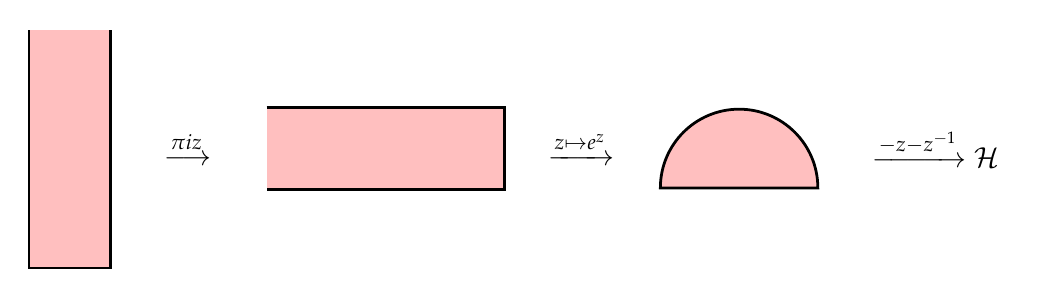
\begin{tikzpicture}[scale=1, transform shape]
        \draw [line width=2pt] (0,3) -- (0,0) -- (1,0) -- (1,3);
        \fill [pink] (0,0) rectangle (1,3);
        \node at (2,1.5) {$\xrightarrow{\pi i z}$};
        \draw [line width=2pt] (3,2) -- (6,2) -- (6,1) -- (3,1);
        \fill [pink] (3,2) -- (6,2) -- (6,1) -- (3,1);
        \node at (7,1.5) {$\xrightarrow{z \mapsto e^z}$};
        \fill [pink] (8,1) arc (180:0:1) -- cycle;
        \draw [line width=1pt] (8,1)  arc (180:0:1) -- cycle;
        \node at (11.5,1.5) {$\xrightarrow{-z-z^{-1}} \mc{H}$};
    \end{tikzpicture}
    \end{center}
    \caption{A sequence of holomorphic bijections}%
    \label{fig:}
    \end{figure}
\end{exm}

Now we will study fractional linear transformaitons in more detail. Let $f \colon \P^1 \to \P^1$ be given by $z \mapsto \frac{az+b}{cz+d}$ with $ad-bc \neq 0$. Then we know that $f$ is a holomorphic bijection and that $\Aut(\P^1) = PGL_2(\C)$. Another important property is the following: given $z_1, z_2, z_3 \in \P^1$ and $w_1, w_2, w_3 \in \P^1$ distinct points, there exists a unique $f$ such that $f(z_j) = w_j$ for $j = 1,2,3$.

To prove existence, we consider the case when $w_1, w_2, w_3 = 0,1,\infty$. Then we simply set 
\[ f(z) = \frac{z - z_1}{z-z_3} \frac{z_2 - z_3}{z_2 - z_1}. \]
To prove uniqueness, we need to do this for the case where $z_1,z_2,z_3 = w_1,w_2,w_3 = 0,1,\infty$. First, fixing $\infty$ means that our transformation is given by $ax + b$. Fixing $0$ means that $b = 0$, and fixing $1$ gives us $a = 1$.

Now let $z_1, z_2, z_3, z_4 \in \P^1$. Then we define the \textit{cross ratio}
\[ CR(z_1, z_2, z_3, z_4) \coloneqq \frac{z_1 - z_3}{z_1 - z_4} \cdot \frac{z_2 - z_4}{z_2 - z_3}. \]
Then if $z_1, z_2, z_3, z_4$ are distinct, the cross ratio is a complex number. Note that if $f$ is the unique M\"obius transformation sending $z_2, z_3, z_4 \mapsto 1,0, \infty$, then $CR(z_1, z_2, z_3, z_4) = f(z_1)$. Therefore, fractional linear transformations preserve the cross ratio. Alternatively, we can compute using brute force.

\begin{prop}
    Fractional linear transformations take circles and lines to circles and lines (for a nicer formulation, these are all circles on $\P^1 = S^2$, where lines are circles passing through $\infty$).
\end{prop}

\begin{proof}
    We will prove that $CR \in \R \P^1$ if and only if $z_1, z_2, z_3, z_4$ lie on a circle or a line. To see this, write $\arg\qty(\frac{z_1-z_3}{z_1-z_4}) = \alpha$ or $-(\pi-\alpha)$. Then $\arg(CR) = 0$ if $z_1, z_2$ lie on the same side of the line connecting $z_3, z_4$ and $\pi$ if they lie on opposite sides, so $CR \in \R$. 

    Conversely, if we fix the circle passing through $z_2, z_3, z_4$, then $z_1 \in C$ if and only if $\arg(CR) = 0$ or $\arg(CR) = \pi$ if and only if $CR \in \R\P^1$.
\end{proof}

For an alternative proof, we know the result is true for $z \mapsto az$ and $z \mapsto z + b$. Then we can check that the result holds for $z \mapsto \frac{1}{z}$, and finally we see that these transformations generate $PGL_2(\C)$.

\begin{exm}
    We may apply this to conformal mapping problems. Set 
    \[ f(z) = \frac{z-1}{z+1} \frac{i+1}{i-1}. \]
    Then $f(1) = 0, f(i) = 1, f(-i) = \infty$. We also know that $f(\partial D) = \partial \mc{H} = \R\P^1$, and $f(D) = \mc{H}$ because $f(0) = i$.
\end{exm}

\begin{lem}
    Let $U, V \subset \C$ and $f \colon U \to V$ be holomorphic and injectivve. Then $f'(z) \neq 0$ for all $z \in U$ and $f^{-1} \colon f(U) \to U$ is holomorphic.
\end{lem}

\begin{proof}
    Near $z_0$, write $f(z) = w_0 + {(z-z_0)}^m g(z)$, where $g(z_0) \neq 0$. In fact, we can write $f(z) = w_0 + {(h(z))}^m$ because we can locally define an $m$-th root of $g$. Then near $z_0$, we see that $f$ is given as the composition
    \[ D \xrightarrow{h} \C \xrightarrow{z \mapsto w_0 + z^m} \C \qquad z_0 \mapsto 0 \mapsto w_0. \]
    Then if $m \geq 2$, the map $z \mapsto z^m$ is not injective near $0$, so $f$ is not injective near $z_0$. Finally, $f^{-1}$ is holomorphic by the inverse function theorem.
\end{proof}

\begin{thm}[Inverse function theorem]
    Let $F \colon U \to \R^2$ and $p \in U$ such that $\det (DF(p)) \neq 0$. Then there exist open neighborhoods $p \in U' \subset U$ and $F(p) \in V \subset \R^2$ such that $F \colon U' \to V$ is a bijection with $F^{-1}$ differentiable and $DF^{-1}(F(p)) = {DF(p)}^{-1}$.
\end{thm}

\begin{lem}[Schwarz]
    Let $D$ be the unit disk and $f \colon D \to D$ be holomorphic such that $f(0) = 0$. Then
    \begin{enumerate}
        \item For all $z \in D$, $\abs{f(z)} \leq \abs{z}$;
        \item If there exists $z_0 \in D$ such that $\abs{f(z_0)} = \abs{z_0}$, then $f$ is a rotation.
        \item $\abs{f'(0)} \leq 1$ with equality if and only if $f$ is a rotation.
    \end{enumerate}
\end{lem}

\begin{proof}
    Consider the function $g(z) = \frac{f(z)}{z}$. Then if $f(z) = a_0 + a_1 z + a_2 z^2 + \cdots$, we know $a_0 = f(0) = 0$, so $g(z) = a_1 + a_2 z + a_3 z^2 + \cdots$ is holomorphic on $D$. Then we apply the maximum principle to $g$, and we note that $\abs{g(z)} < \frac{1}{r}$ for $\abs{z} = r < 1$, so $\abs{g(z)} < \frac{1}{r}$ for $\abs{z} \leq r$. Allowing $r \to 1$ from below, we see that $\abs{g(z)} \leq 1$ for all $z \in D$ and therefore $\abs{f}(z) \leq \abs{z}$.

    Now if $\abs{f(z)} = \abs{z}$ for some $z_0 \in D$, then $g(z)$ must be constant and therefore $f(z) = cz$ with $\abs{c} = 1$. Finally, we note that $g(0) = f'(0)$ and then if $g(0) = 1$, we see that $f$ is a rotation by the second part.
\end{proof}

Now we are ready to consider automorphisms of the disk and upper half plane. In the case of the disk, we have two kinds of automorphisms:
\begin{enumerate}
    \item Rotations $z \mapsto e^{i\theta}z$;
    \item \textit{Blaschke factors} $\psi_{\alpha}(z) = \frac{\alpha - z}{1 - \ol{\alpha}z}$, where $\alpha \in D$. We can check that $\psi_{\alpha}(\partial D) = \partial D$. 
\end{enumerate}

\begin{prop}
    Every automorphism of the disk is of the form
    \[ z \mapsto e^{i\theta} \frac{\alpha - z}{1 - \ol{\alpha} z} \]
    for some $\theta, \alpha$.
\end{prop}

\begin{proof}
    Given an automorphism $f \colon D \to D$, then the map $f \circ \psi_{\alpha}$ fixes the origin and is a rotation by the Schwarz lemma because it also fixes $\alpha$. Therefore, $f = r \circ \psi_{\alpha}^{-1} = r \circ \psi_{\alpha}$, where $r$ is some rotation.
\end{proof}

Note that if $f \colon D \to D$ is an automorphism with $f(0) = 0$, then the Schwarz lemma implies that $\abs{f(z)} \leq \abs{z}$ and $\abs{f^{-1}(z)} \leq \abs{z}$ and therefore $\abs{z} = \abs{f(z)}$ and therefore $f$ is a rotation.o

Now we want to study automorphisms of $\mc{H}$. We know that $\mc{H}, D$ are isomorphic, so $\Aut D = \Aut \mc{H}$.

\begin{thm}
    We have $\Aut(\mc{H}) \cong PSL_2(\R)$.
\end{thm}

\begin{proof}
    Let $f(z) = \frac{az + b}{cz + d}$. Then we see that
    \[ \Im(f(x+iy)) = \frac{ay(cx+d) - cy(ax+b)}{{(cx+d)}^2 + y^2} = \frac{(ad-bc)y}{{(cx+d)}^2 + y^2} > 0, \]
    and thus we require $ad - bc > 0$. Therefore we have $PSL_2(\R) \subset \Aut \mc{H}$.

    Now we prove surjectivity. First, we note that $PSL_2(\R)$ acts transitively on $\mc{H}$. First, if $b \in \R$, $z \mapsto z + b$ preserves $\mc{H}$ and if $\lambda > 0$, $z \mapsto \lambda z$ preserves $\mc{H}$. Next, we consider the effect of rotation $ \begin{psmallmatrix}
        \cos \varphi & - \sin \varphi \\ \sin \varphi & \cos \varphi
    \end{psmallmatrix}$. But we can compute that
    \[ \mqty(-1 & i \\ 1 & i) \mqty( \cos \varphi & - \sin \varphi \\ \sin \varphi & \cos \varphi ) = \mqty(-e^{i\varphi} & ie^{-i\varphi} \\ e^{i\varphi} & ie^{i\varphi}) = e^{i\varphi} \mqty(e^{2i\varphi} & \\ & 1) \mqty(-1 & i \\ 1 & i). \]
    To finish, we show that given $f \colon \mc{H} \to \mc{H}$, then $f \in PSL_2(\R)$. Suppose $f(\alpha) = i$. Then there exists $g \in G$ such that $g(i) = \alpha$. Then $g \circ f$ fixes $i$, so $F \circ g \circ f \circ F^{-1}$ fixes $0$ and is thus a rotation. Therefore there exists $h \in G$ such that $F \circ g \circ f \circ F^{-1} = F \circ h \circ F^{-1}$, so $g \circ f = h$ and $f = h \circ g^{-1}$.
\end{proof}

\section{Riemann Mapping Theorem}%
\label{sec:riemann_mapping_theorem}

Our goal in this section is to prove the Riemann mapping theorem.

\begin{thm}
    Let $\Omega \subset \C$ be open and $\qty{f_n}_{n=1}^{\infty}$ be a sequence of holomorphic functions $f_n \colon \Omega \to \C$ which converges uniformly to $f$ on every compact subset $K \subset \Omega$. Then $f$ is holomorphic.
\end{thm}

\begin{proof}
    Let $D = \qty{z \in \C \mid \abs{z - z_0} < r} \subset \Omega$. Then $f_n$ being holomorphic implies that $\int_{\gamma} f_n(z) \dd{z} = 0$ for all closed curves $\gamma$ in $D$. Because $f_n \to f$ uniformly, we have
    \[ \int_{\gamma} f(z) \dd{z} = \lim_{n \to \infty} \int_{\gamma} f_n(z) \dd{z} = 0. \]
    Also we know that $f$ is continuous. Now we define
    \[ F(z) = \int_{\gamma_z} f(w) \dd{w} \qquad F \colon \Omega \to \C. \]
    Here, $\gamma_z$ is a path from $z_0$ to $z$ for a fixed basepoint $z_0$. Then $F$ is well-defined and $F' = f$, so $f$ is holomorphic.
\end{proof}

\begin{lem}
    Let $\Omega \subset \C$ be open and $f_n \colon \Omega \to \C$ be holomorphic. Suppose that $f_n \to f$ uniformly on compact sets. Then $f_n' \to f'$ uniformly on compact sets.
\end{lem}

\begin{proof}
    Let $K' = \qty{z \in \C \mid d(z,K) leq r}$ for some $r \in \R$ such that $K' \subset \Omega$. Then we know $f_n \to f$ uniformly on $K'$, and we will use this to show that $f_n' \to f'$ uniformly on $K$. Using the Cauchy integral formula to some holomorphic function $h$, we have
    \[ h'(z) = \frac{1}{2 \pi i} \int_{\gamma} \frac{h(w)}{{(w-z)}^2} \dd{w}, \]
    so then we can bound
    \[ \abs{h'(z)} \leq \frac{1}{2\pi} 2 \pi r \cdot \frac{1}{r^2} \sup_{w \in \gamma} \abs{h(w)} = \frac{1}{r} \sup_{w \in \gamma} \abs{h(w)}. \]
    Applying this to $h = f_n - f$, we see that for all $\ep > 0$, there exists $N \in \N$ such that $\abs{f_n(w) - f(w)} < \ep$ on $K'$ for all $n > N$, and this implies that $\abs{f_n'(z) = f'(z)} < \frac{1}{r} \ep$ on $K$.
\end{proof}

Now let $\Omega \subset \C$ be open and $\mc{F}$ be a set of holomorphic functions on $\Omega$. We say that $\mc{F}$ is \textit{normal} if every sequence in $\mc{F}$ has a subsequence which converges uniformly on compact sets to some function $f \colon \Omega \to \C$. We say that $\mc{F}$ is \textit{uniformly bounded on compact sets} if for all compact $K \subset \Omega$, there exists $M \in \R$ such that $\abs{f(z)} \leq M$ for all $f \in \mc{F}, z \in K$. Finally, we say that $\mc{F}$ is \textit{equicontinuous} on a compact set $K \subset \Omega$ if for all $\ep > 0$ there exists $\delta > 0$ such that $\abs{f(z) - f(w)} < \ep$ for all $z,w \in K$ such that $\abs{z - w} < \delta$ and $f \in \mc{F}$.

\begin{thm}[Montel]
    Let $\mc{F}$ be a family of holomorphic functions on $\Omega \subset \C$ that is uniformly bounded on comact sets. Then
    \begin{enumerate}
        \item $\mc{F}$ is equicontinuous on compact sets;
        \item $\mc{F}$ is normal.
    \end{enumerate}
\end{thm}

\begin{rmk}
    The first part uses holomorphicity, and the second part uses a general fact, the Arzel\`a-Ascoli theorem.
\end{rmk}

\begin{exm}
    Let $f_n(z) = z^n$. Then $\mc{F} = \qty{f_n}$ is \textbf{not} equicontinuous on $K = [0,1]$. In fact, $\abs{f_n(z) - f_n(1)} = \abs{z^n - 1} \to 1$ as $n \to \infty$ for $z \in (0,1)$.
\end{exm}

\begin{exm}
    Let $\mc{F} = \qty{f_n(z) = \sin(nz)}$. Then $\mc{F}$ is \textbf{not} equicontinuous on $K = [0,1]$ because $f_n\qty(\frac{\pi}{2n}) = 1$, but $f_n(0) = 0$.
\end{exm}

\begin{proof}[Proof of Montel's theorem]\leavevmode
    \begin{enumerate}
        \item We will use the Cauchy integral formula to bound $\abs{f(z) - f(w)}$. Let $K \subset \Omega$ be compact and choose $r > 0$ such that $K' = \qty{z \in \C \mid d(z,K) \leq 2r} \subset \Omega$. Given $z,w \in K$ such that $\abs{z - w} < r$, we will let $\gamma$ be the circle with center $z$ and radius $2r$. We know $\gamma \subset K'$. Now we have
            \begin{align*}
                f(z) - f(w) = \frac{1}{2 \pi i} \int_{\gamma} \frac{f(u)}{u-z} - \frac{f(u)}{u-w} \dd{u} = \frac{1}{2 \pi i} \int_{\gamma} f(u) \mqty(\frac{1}{u-z} = \frac{1}{u-w} \dd{u}).
            \end{align*}
            Then we can bound
            \[ \abs{\frac{1}{u-z} - \frac{1}{u-w}} = \abs{\frac{z-w}{(u-z)(u-w)}} \leq \frac{\abs{z-w}}{2r \cdot r} = \frac{1}{2r^2} \abs{z-w}, \]
            so 
            \[ \abs{f(z) - f(w)} \leq \frac{1}{2\pi} \cdot 2 \pi \cdot 2r \cdot \frac{1}{2r^2} \abs{z-w} \sup_{u \in \gamma} \abs{f(u)} = \frac{1}{r} \abs{z-w} \cdot M, \]
            where $\abs{f(u)} \leq M$ for all $u \in K, f \in \mc{F}$. Therefore $\mc{F}$ is equicontinuous on $K$.
        \item Let $K \subset \Omega$ be compact and $f_n$ be a sequence in $\mc{F}$. First let ${(w_j)}_{j=1}^{\infty}$ be a sequence in $K$ which is dense. To construct such a sequence, recall that 
            \[ K = \bigcup_{x \in K} D\qty(x, \frac{1}{n}) \cap K. \]
            By compactness, there exists a finite $S_n \subset K$ such that $K = \bigcup_{x \in S_n} D(x, 1/n) \cap K$, and now we can take $S = \bigcup_{n \geq 1} S_n$ and obtain a countable dense subset. 

            Now we will use a ``diagonal argument.'' If $f_n$ is uniformly bounded, then the sequence $f_n(w_1)$ has a convergent subsequence $f_{n,1}(w_1)$. Continuing, there exists a subsequence $\qty{f_{n,2}}$ of $\qty{f_{n,1}}$ such that $f_{n,2}(w_2)$ converges. For each $m \in \N$, there exists a subsequence $\qty{f_{n,m}}$ of $\qty{f_n}$ such that $f_{n,m}(w_k)$ converges for all $k \leq m$. Now take $g_n = f_{n,n}$. This is a subsequence of $\qty{f_n}$ such that $g_n(w_k)$ converges for all $k \in \N$. If $z \in K$, then 
            \[ \abs{g_n(z) - g_m(z)} \leq \abs{g_n(z) - g_n(w_j)} + \abs{g_n(w_j) - g_m(w_j)} + \abs{g_m(z) - g_m(w_j)} \]
            by the triangle inequality. 

            Now carefully, we know that given $\ep > 0$ there exists $\delta > 0$ such that $\abs{g_n(z) - g_n(w)} < \ep$ whenever $\abs{z-w} < \delta$ and $z,w \in K$. Because $K$ is compact, $K \subseteq \bigcup_{j=1}^J D(w_j, \delta)$ for some $J \in \N$. Given $z \in K$, there exists $w_j$ such that $\abs{z-w_j} < \delta$, so $\abs{g_n(z) - g_m(z)} < \ep$. Now for $n,m$ large, we have $\abs{g_n(z) - g_m(z)} < 3 \ep$ because there exists $N \in \N$ such that $\abs{g_n(w_j) - g_m(w_j)} < \ep$ for $n,m \geq N$. Therefore $g_n(z)$ converges uniformly for all $z \in K$.

            For all compact sets $K$, we need another diagonal argument. There exists an exhaustion 
            \[ K_1 \subset K_2 \subset \cdots \subset \Omega \]
            such that $K_{\ell}$ is contained in the interior of $K_{\ell + 1}$ and for all $K \subset \Omega$ compact, $K \subset K_{\ell}$ for some $\ell$. For example, set 
            \[ K_{\ell} = \qty{z \in \Omega \mid d(z, \C \setminus \Omega) \geq \frac{1}{\ell}} \cap \qty{z \in \C \mid \abs{z} \leq \ell}. \]

            Finally, given a sequence $f_n \in \mc{F}$, we have a subsequence $g_{n,1}$ converging uniformly on $K$, a subsequence $g_{n,2}$ of $g_{n,1}$ converging uniformly on $K_2$, and now the sequence $h_n = g_{n,n}$ converges uniformly on all $K_{\ell}$ and hence on all $K$. \qedhere
    \end{enumerate}
\end{proof}

We are now ready to prove the Riemann mapping theorem, and in fact we have a stronger statement.

\begin{thm}[Riemann mapping theorem]
    Let $\Omega \subset \C$ be a nonempty proper simply-connected open subset of $\C$. Fix $z_0 \in \Omega$. Then there exists a unique holomorphic bijection $F \colon \Omega \to B$ such that $F(z_0) = 0, F'(z_0) \in \R_{>0}$.
\end{thm}

\begin{rmk}
    Uniqueness follows from the Schwarz lemma. If we have $F_1, F_2$ two such functions, then $G = F_2 \circ F_1^{-1} \colon D \to D$ has $G(0) = 0$ and $G'(0) \in \R_{>0}$, so $G(z) = e^{i\theta} z$. But then $G'(0) = e^{i \theta} \in \R_{>0}$, so $G = \mr{id}$.
\end{rmk}

\begin{proof}
    Consider 
    \[ \mc{F} = \qty{g \colon \Omega \hookrightarrow D \mid g(z_0) = 0, g'(z_0) \in \R_{>0}}. \]
    By construction, $\mc{F}$ is uniformly bounded and thus normal.

    First, we show that $\mc{F}$ is nonempty. By assumption $\Omega \neq \C$, so let $a \in \C \setminus \Omega$. Then we can define $f \colon \Omega \to \C$ defined by $z \mapsto \log(z-a)$. Then $e^{f(z)} = z-a$. Note that $f$ is injective and recall that $e^{w + 2\pi i k} = e^w$ for all $k \in \Z$. Take $w_0 \in f(\Omega)$. Then $f(\Omega)$ is open, so $D(w_0, \delta) \subset f(\Omega)$ for some $\delta > 0$. Then we see that $D(w_0 + 2 \pi i, \delta) \cap f(\Omega) = \emptyset$, so we can take
    \[ g(z) = \frac{1}{f(z) - (w_0 + 2 \pi i)}, \]
    and we have $\abs{g} < \frac{1}{\delta}$. Because $f$ is injective, $g$ is injective. Composing with translation and rotation, we can assume that $g(z_0) = 0$ and $g'(z_0) \in \R > 0$. Composing with scaling, we may assume that $\abs{g} < 1$, so $g \in \mc{F}$.

    Now let $g_n$ be a sequence in $\mc{F}$ such that $g_n'(z_0) \to \sup_{g \in \mc{F}} g'(z_0)$. By Montel's theorem, $g_n \to g$ uniformly on compact sets for some $g \colon \Omega \to \C$. then $g$ is holomorphic and $g_n' \to g'$ uniformly on compact sets, so in particular $g'(z_0) = \sup_{h \in \mc{F}} h'(z_0)$. We will prove that $g$ is a bijection. To prove injectivity, fix $z_1, z_2 \in \Omega$. Define $\wt{g}_n(z) = g_n(z) = g_n(z_1)$ and $\wt{g}(z) = g(z) - g(z_1)$. Then $\wt{g}_n(z) \neq 0$ for $z \neq z_1$. Given $z_2 \in \Omega \setminus \qty{z_1}$, there exists $\delta > 0$ such that $\wt{g}(z) \neq 0$ for $0 < \abs{z - z_2} \leq \delta$. Also assume $\abs{z_1 - z_2} > \delta$. Let $\gamma = \qty{z \mid \abs{z-z_2} = \delta}$. Then we have
    \[ \frac{1}{2 \pi i} \int_{\gamma} \frac{\wt{g}'(z)}{\wt{g}(z)} \dd{z} = \lim_{n \to \infty} \frac{1}{2 \pi i} \frac{\wt{g}_n'(z)}{\wt{g}_n(z)} \dd{z} = \lim_{n \to \infty} 0 = 0, \]
    so $g$ is injective.

    We will prove surjectivity by contradiction. Suppose there exists $\alpha \in D \setminus g(\Omega)$. Define $U = \psi_{\alpha}(g(\Omega))$ and $U \subset D$ is open, simply connected, and $0 \notin U$. We can define $k \colon U \to D$ by $k(z) = \sqrt{z} = e^{\frac{1}{2} \log z}$. Now we can set $G = r_{\theta} \circ \psi_{\beta} \circ k \circ \psi_{\alpha} \circ g$, where $\beta = k(\alpha)$. Equivalently, we have $g = \psi_{\alpha} \circ\ell \circ \psi_{\beta} \circ r_{-\theta} \circ G$, and set $\psi_{\alpha} \circ \ell \circ \psi_{\beta} \circ r_{-\theta} = L$. Then $L \colon D \to D$ fixes $0$ and is not a rotation, so $\abs{L'(0)} < 1$. Therefore $\abs{g'(z_0)} = \abs{L'(0) \cdot G'(0)} < \abs{G'(z_0)}$ by the chain rule, which is a contradiction.
\end{proof}

\section{Elliptic Functions}%
\label{sec:elliptic_functions}

Recall that meromorphic functions on $\P^1$ are the rational functions. We would like to study meromorphic functions on the complex torus $X = \C/\Lambda$, where $\Lambda = \Z \omega_1 + \Z \omega_2$ for $0 \neq \omega_1, \omega_2 \in \C$ with $\omega_2 / \omega_! \notin \R$. Equivalently, we want to consider doubly periodic meromorphic functions on $\C$.

\begin{lem}
    If $f$ is holomorphic on $X$, then $f$ is constant.
\end{lem}

\begin{proof}
    Clearly, $f$ is given by values on a parallelogram, so $f$ is bounded and therefore constant.
\end{proof}

\begin{rmk}
    If $X$ is a compact Riemann surface, then all holomorphic functions $f \colon X \to \C$ are constant. This is because $\abs{f}$ is bounded and attains its maximum on some chart, so it must be constant.
\end{rmk}

\begin{lem}
    Let $f$ be meromorphic on $\C / \Lambda$. Then $f$ has at least $2$ poles.
\end{lem}

\begin{proof}
    Integrating around the boundary of the parallelogram, we see that 
    \[ 0 = \int_{\gamma} f(z) \dd{z} = 2 \pi i \sum_{p} \Res_p f \]
    because $\sum \Res_p f = 0$ by an analog of the residue theorem.
\end{proof}

\begin{rmk}
    There is a suitably generalized version of the residue theorem for any compact Riemann surface. First, define a meromorphic $1$-form $\omega$. Choose charts $\varphi_i \colon U_i \simeq V_i$. On each $V_i$, we have a form $f_i(z) \dd{z}$ with $f_i(z)$ meromorphic. Then compatibility with transitions $g_{ij}$ is given by
    \[ f_i(z) = f_j(g_{ij}(z)) g_{ij}'(z) \dd{z}, \]
    and thus we can define the integral of $\omega$ along a curve $\gamma \subset X$. Now the residue theorem says that if $X$ is a compact Riemann surface and $\omega$ is a meromorphic $1$-form on $X$, then $\sum_{p\ \text{pole}} \Res_p \omega = 0$.

    For example, on $X = \P^1$, we can consider $\omega = \frac{1}{z} \dd{z}$. Then on the second chart, we see that $\omega = w \cdot \dd\qty(\frac{1}{w}) = -\frac{1}{w} \dd{w}$. Then we see that $\sum_p \Res_p \omega = 1 + (-1) = 0$.

    To prove the residue theorem, triangulate $X$ such that each triangle is contained in some $U_i$. Then $\sum_{\Delta_i} \int_{\partial \Delta_i} \omega = 0 = 2 \pi i \sum_p \Res_p \omega$.
\end{rmk}

\begin{cor}
    Let $f$ be meromorphic on a compact Riemann surface $X$. Then the number of zeroes of $f$ equals the number of poles of $f$.
\end{cor}

\begin{proof}
    Given $f$, we may define the meromorphic form $\dd{f}$. Then we can consider the meromorphic form $\omega = \frac{\dd{f}}{f}$. Then by the residue theorem we see that
    \[ 0 = \sum_p \Res_p \omega = \# \qty{\text{zeroes}} - \# \qty{\text{poles}}. \qedhere \]
\end{proof}

The geometric meaning is that if $f \colon X \to \P^1$ is holomorphic, then for all $\alpha$, $f^{-1}(\alpha) = \deg f$, counting multiplicity.

Now we will define an explicit meromorphic function $\wp$ on $\C/\Lambda$ with a unique double pole at $0 \in X$. Equivalently, $\wp \colon \C \to \P^1$ has a double pole at each point in $\Lambda$. Define
\[ \wp(z) \coloneqq \frac{1}{z^2} + \sum_{\omega \in \Lambda \setminus \qty{0}} \frac{1}{{(z+\omega)}^2} - \frac{1}{\omega^2} \]
because the first attempt $\wp(z) = \sum_{\omega \in \Lambda} \frac{1}{{(z+\omega)}^2}$ doesn't converge.

\begin{lem}
    The function $\wp(z)$ converges absolutely and uniformly on compact sets $K \in \C \setminus \Lambda$ and has a double pole at each $\omega \in \Lambda$.
\end{lem}

\begin{proof}
    First note that
    \[ \abs{\frac{1}{{(z+\omega)}^2} - \frac{1}{\omega^2}} = \abs{\frac{z^2 + 2z\omega}{{(z+2)}^2 \omega^2}} \leq C \cdot \frac{1}{\abs{\omega}^3} \]
    for $\abs{\omega}$ large and $z$ bounded. Now we show that $\sum_{0 \neq \omega \in \Lambda} \frac{1}{\abs{\omega}^3}$ converges. First, we know that $\omega = x_1 \omega_1 + x_2 \omega_2$. Then for any $x_1, x_2 \in \R$, we know $\abs{x_1 \omega_1 + x_2 \omega_2} \geq C \sqrt{x_1^2 + x_2^2}$. This is because the function $f(x_1, x_2) = \abs{x_1 \omega_1 + x_2 \omega_2}$ satisfies $f(\lambda \mathbf{x}) = \lambda f(\mathbf{x})$. Therefore if $\norm{x} = 1$, we know $f$ lands in the positive reals and has a positive minimum. Therefore, we have reduced to the case where $\omega_1 = 1, \omega_2 = i$. Now we want to show that
    \[ \sum_{0 \neq \mathbf{x} \in \Z^2} \frac{1}{\sqrt{{(x_1^2 + x_2^2)}^3}} \]
    converges. Using the integral test, we see that
    \begin{align*}
        \sum_{0 \neq (x_1, x_2) \in \Z^2} \frac{1}{{(x_1^2 + x_2^2)}^{\alpha/2}} &\leq C + \int_R \frac{1}{{(x_1^2 + x_2^2)}^{\alpha/2}} \dd{x_1} \dd{x_2} \\
                                                                                 &= C + \int_{0}^{2\pi} \int_1^{\infty} \frac{1}{r^{\alpha}} r \dd{r} \dd{\theta} \\
                                                                                 &= C + 2 \pi \int_1^{\infty} \frac{1}{r^{\alpha - 1}} \dd{r},
    \end{align*}
    and therefore it converges for $\alpha > 2$.
\end{proof}

Now we need to check that $\wp$ is doubly periodic. Here, we simply note that
\[ \wp'(z) = \frac{-2}{z^3} + \sum_{0 \neq \omega \in \Lambda} \frac{-2}{{(z+\omega)}^3} = \sum_{\omega \in \Lambda} \frac{-2}{{(z+\omega)}^3} \]
is doubly periodic, so $\wp(z+\omega) - \wp(z)$ is constant. Now checking $\omega = \omega_1$ and $z = - \frac{1}{2} \omega$, we see that $\wp\qty(\frac{1}{2} \omega) - \wp\qty(-\frac{1}{2} \omega) = 0$ because $\wp$ is even.

\begin{thm}
    We have the differential equation
    \[ {(\wp')}^2 = 4(\wp - \alpha_1)(\wp - \alpha_2)(\wp-\alpha_3) \]
    where $\alpha_1, \alpha_2, \alpha_3 = \wp\qty(\frac{\omega_1}{2}), \wp\qty(\frac{\omega_2}{2}), \wp\qty(\frac{\omega_1 + \omega_2}{2})$.
\end{thm}

\begin{proof}
    We will compute the zeroes and poles of the two sides of the equations and show that they agree. Then their quotient is holomorphic on $X = \C /\Lambda$ and thus constant, so we can compute the constant. Recall that $\wp$ has a pole of order $2$ at $0$ and $\wp'$ has a pole of order $3$ at $0$. Next, $\wp$ is even so $\wp'$ is odd. Then we know that 
    \[ \wp'\qty(\frac{\omega}{2}) = \wp'\qty(\frac{\omega}{2} - \omega) = \wp'\qty(-\frac{\omega}{2}) = -\wp'\qty(\frac{\omega}{2}) \]
    and thus $\wp'\qty(\frac{\omega}{2}) = 0$. Then $\wp - \wp\qty(\frac{\omega}{2})$ has a zero of order $2$ at $\frac{\omega}{2}$.

    Now to compute the constant, we use the Laurent series at the origin. We know that
    \begin{align*}
        \wp = \frac{1}{z^2} + \cdots \qquad \wp' = \frac{-2}{z^3} + \cdots \qquad {(\wp')}^2 = \frac{4}{z^6} + \cdots \qquad \prod_{i=1}^3(\wp - \alpha_i) = \frac{1}{z^6} + \cdots,
    \end{align*}
    and thus ${(\wp')}^2 = 4 \prod_{i=1}^3 (\wp - \alpha_i)$.
\end{proof}

Now we have the identity
\[ \int \frac{\dd{w}}{\sqrt{(w-\alpha_1)(w-\alpha_2)(w-\alpha_3)}} = \int \frac{\wp'(z) \dd{z}}{\wp'(z)} = z = \wp^{-1}(w), \]
where $w = \wp(z)$ and ${(\wp')}^2 = \prod_{i=1}^3 (\wp - \alpha_i)$.

\begin{thm}
    Every meromorphic function on $X = \C / \Lambda$ is a rational function of $\wp, \wp'$. This means that the field of meromorphic funcions on $X$ is given by
    \[ \C(X) = k(\C[x,y]/(y^2 - 4(x-\alpha_1)(x-\alpha_2)(x-\alpha_3))) = \C(x)[y]/(y^2 - 4(x-\alpha_1)(x-\alpha_2)(x-\alpha_3)). \]
    Therefore we can write $f \in \C(x)$ uniquely as $a(\wp) + b(\wp) \wp'$ for $a,b \in \C(x)$.
\end{thm}

\begin{proof}
    First suppose that $f$ is \textbf{even}. We will show that $f$ is rational in $\wp$. We may assume that $f$ has no poles on $\Lambda \subset \C$ up to replacing $f$ by $\wp^{-m} f$. Now if we write down a function with the same zeroes and poles and is a rational function of $\wp$. Recall that $\wp(z) - \wp(a)$ has zeroes $\begin{cases} a, -a & a \neq -a \\ a\ (\text{twice}) & a \in \frac{1}{2} \Lambda \end{cases}$. But then for our function $f$, because $f$ is even, the zeroes and poles of $f$ come in pairs $a, -a$ or $a \in \frac{1}{2} \Lambda$ has even multiplicity. Then $f$ has the same poles as
    \[ \frac{\prod (\wp - \wp(a_i))}{\prod (\wp - \wp(b_j))} \]
    for some $a_i, b_j \in \C$. Note that $\wp$ has a pole of multiplicity $2$ at $0 \in X$ and no other poles and $f$ has no zero or pole at $0 \in X$ by assumption. But we are fine because $\# \qty{a_i} = \# \qty{b_j}$.

    In the general case, suppose $f$ is meromorphic on $X$. Then write 
    \[ f(z) = \frac{f(z) + f(-z)}{2} + \frac{f(z) - f(-z)}{2}. \]
    Then if $g$ is odd, $\frac{g}{\wp'}$ is even and thus rational in $\wp$, so we obtain the desired description.
\end{proof}

Now we can give a geometric description of this. Note that $X = \C/\Lambda \xrightarrow{\wp} \P^1$ has degree $2$. It has branch points at $a_1 = \wp\qty(\frac{\omega_1}{2}, a_2 = \wp\qty(\frac{\omega_2}{2})), a_3 = \wp\qty(\frac{\omega_1 + \omega_2}{2}), \infty$. Now we have a map
\[ X \xrightarrow{\wp, \wp'}{\sim} (y^2 = (x-a_1)(x-a_2)(x-a_3)) \subset \P^2. \]
Now we can make two branch cuts, then expand the branch cuts into circles, and obtain half of a torus. Gluing two halves together, we obtain the torus. There is an involution $(x,y) \mapsto (x,-y)$ that exchanges the two sheets of the torus. As a picture, it looks like
\begin{figure}[H]
\begin{center}
\begin{tikzpicture}[scale=1, transform shape]
    \draw (0,0) ellipse (3 and 1.5);
    \node[circle,fill=black,inner sep=0pt, minimum size=3pt] (A) at (-2,0) {};
    \node[circle,fill=black,inner sep=0pt, minimum size=3pt] (B) at (-1,0) {};
    \node[circle,fill=black,inner sep=0pt, minimum size=3pt] (C) at (1,0) {};
    \node[circle,fill=black,inner sep=0pt, minimum size=3pt] (D) at (2,0) {};
    \draw (A) -- (B);
    \draw (C) -- (D);
    \node at (3.5,0) {$\overset{2:1}{ \longleftarrow }$};
    \draw (7,0) ellipse (3 and 1.5);
  \begin{scope}
    \clip (7,-1.8) ellipse (3 and 2.5);
    \draw (7,2.2) ellipse (3 and 2.5);
  \end{scope}
  \begin{scope}
    \clip (7,2.2) ellipse (3 and 2.5);
    \draw (7,-2.2) ellipse (3 and 2.5);
  \end{scope}
\end{tikzpicture}
\end{center}
\caption{Branched cover of sphere by torus}%
\label{fig:}
\end{figure}

\section{Winding Numbers}%
\label{sec:winding_numbers}

Let $\gamma \subset \C$ be a closed path. For $a \in \C \setminus \gamma$, define the \textit{winding number}
\[ n(\gamma, a) \coloneqq \frac{1}{2 \pi i} \int_{\gamma} \frac{1}{z-a} \dd{z}. \]
This is reasonable because if we consider the covering space $\R \to S^1 = \R/2 \pi \Z$. Then if we write $z(t) = a + r(t) e^{i \theta(t)}$, we have
\begin{align*}
    n(\gamma, a) &= \frac{1}{2 \pi i} \int_0^1 \dd(\log(z(t) - a)) \\
                 &= \frac{1}{2 \pi i} \int_0^1 \dd(\log r(t)) + i \dd(\theta(t)) \\
                 &= \frac{1}{2 \pi} (\theta(1) - \theta(0)).
\end{align*}

\begin{thm}\leavevmode
    \begin{enumerate}
        \item For all $a, \gamma$, we have $n(\gamma, a) \in \Z$.
        \item If $a, b$ lie in the same component of $\C \setminus \gamma$, then $n(\gamma, a) = n(\gamma(b))$.
        \item If $a$ lies in the unbounded component of $\C \setminus \gamma$, then $n(\gamma, a) = 0$.
        \item If $\gamma, \delta$ are homotopic in $\C \setminus \qty{a}$, then $n(\gamma, a) = n(\delta, a)$.
    \end{enumerate}
\end{thm}

\begin{proof}\leavevmode
    \begin{enumerate}
        \item Let $z \colon [0,1] \to \gamma \subset \C$. Then define
            \[ g(t) \coloneqq \int_0^t \frac{z'(s)}{z(s) - a} \dd{s}. \]
            Then we see that ${((z(t) - a)e^{-g(t)})}' = z'(t) e^{-g(t)} - (z(t)-a) g'(t) e^{-g(t)} = 0$. But then $e^{g(1)} = e^{g(0)} \equiv c \cdot (z(0)-a)$, so $g(1) - g(0) \in 2 \pi i \Z$. Therefore $n(\gamma, a) \in \Z$.
        \item We know that the winding number $\C \setminus \gamma \to \Z \subset \C$ is continuous, so it must be locally constant.
        \item Note that 
            \[ n(\gamma, a) = \frac{1}{2 \pi i} \int_{\gamma} \frac{1}{z-a} \dd{z} \]
            so as $a \to \infty$, $n(\gamma, a) \to 0$, but it must be constant, so $n(\gamma, a) = 0$.
        \item Note that $\frac{1}{z-a}$ is holomorphic on $\C \setminus \qty{a}$. Then the desired result follows from Theorem 2.7.1. \qedhere
    \end{enumerate}
\end{proof}

We can compute winding numbers using \textit{Alexander numbering}. 
\begin{figure}[H]
\begin{center}
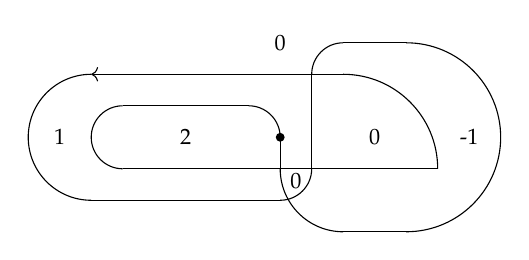
\begin{tikzpicture}[scale=0.8, transform shape]
    \fill (0,0) circle (2pt);
    \draw (0,0) arc (0:90:0.5);
    \draw (-0.5,0.5) -- (-2.5,0.5);
    \draw (-2.5,0.5) arc (90:270:0.5);
    \draw (-2.5,-0.5) -- (2.5,-0.5);
    \draw (2.5,-0.5) arc (0:90:1.5);
    \draw[->] (1,1) -- (-3,1);
    \draw (-3,1) arc (90:270:1);
    \draw (-3,-1) -- (0,-1);
    \draw (0,-1) arc (-90:0:0.5);
    \draw (0.5,-0.5) -- (0.5,1);
    \draw (1,1.5) arc (90:180:0.5);
    \draw (1,1.5) -- (2,1.5);
    \draw (2,-1.5) arc (-90:90:1.5);
    \draw (0,-0.5) arc (180:270:1);
    \draw (0,0) -- (0,-0.5);
    \draw (1,-1.5) -- (2,-1.5);
    \node (A) at (-3.5,0){1};
    \node (B) at (-1.5,0){2};
    \node (C) at (0,1.5){0};
    \node (D) at (3,0){-1};
    \node (E) at (0.25,-0.7){0};
    \node (F) at (1.5,0){0};
\end{tikzpicture}
\end{center}
\caption{Winding numbers}%
\label{fig:}
\end{figure}
We know the winding number vanishes on the unbounded component, and given $\alpha \uparrow \beta$, we have $n(\gamma, \alpha) = n(\gamma, \beta) + 1$ because in the diagram
\begin{figure}[H]
\begin{center}
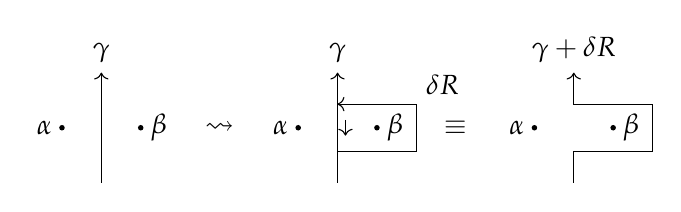
\begin{tikzpicture}[scale=1, transform shape]
    \node [left] at (0,0) {$\alpha$};
    \fill (0,0) circle (1pt);
    \draw[->] (0.5,-0.7) -- (0.5,0.7);
    \node [above] at (0.5, 0.7) {$\gamma$};
    \node [right] at (1,0) {$\beta$};
    \fill (1,0) circle (1pt);
    \node at (2,0) {$\rightsquigarrow$};
    \node [left] at (3,0) {$\alpha$};
    \fill (3,0) circle (1pt);
    \draw[->] (3.5,-0.7) -- (3.5,0.7);
    \node [above] at (3.5, 0.7) {$\gamma$};
    \node [right] at (4,0) {$\beta$};
    \fill (4,0) circle (1pt);
    \draw[->] (3.5,-0.3) -- (4.5,-0.3) -- (4.5,0.3) -- (3.5,0.3);
    \draw[->] (3.6, 0.1) -- (3.6,-0.1);
    \node [above right] at (4.5,0.3) {$\delta R$};
    \node at (5,0) {$\equiv$};
    \node [left] at (6,0) {$\alpha$};
    \fill (6,0) circle (1pt);
    \node [right] at (7,0) {$\beta$};
    \fill (7,0) circle (1pt);
    \draw[->] (6.5, -0.7) -- (6.5,-0.3) -- (7.5, -0.3) -- (7.5, 0.3) -- (6.5,0.3) -- (6.5,0.7);
    \node [above] at (6.5, 0.7) {$\gamma + \delta R$};
\end{tikzpicture}
\end{center}
\caption{Pictoral proof of Alexander numbering}%
\label{fig:}
\end{figure}
we have $n(\gamma, \alpha) = n(\gamma + \delta R, \alpha) = n(\gamma + \delta R, \beta) = n(\gamma, \beta) + 1$.

\begin{thm}[Cauchy]
    Let $f \colon \Omega \to \C$ and $\gamma \subset \Omega$ be a closed curve such that $n(\gamma, a) \neq 0$ for all $a \in \C \setminus \Omega$. Then
    \[ \int_{\gamma} f(z) \dd{z} = 0. \]
\end{thm}

\begin{cor}[General Residue Theorem]
    Let $\Omega \subset \C$ be open and $S \subset \Omega$ be a discrete set. Suppose $f \colon \Omega \setminus S \to \C$ is holomorphic and $\gamma \subset \Omega \setminus S$ is a closed curve. Then
    \[ \int_{\gamma} f(z) \dd{z} = 2 \pi i \sum_{a \in S} n(\gamma, a) \Res_a f. \]
\end{cor}

\begin{rmk}
    The assumption that $S$ is discrete implies that there are only finitely many $a \in S$ with nonzero winding number.
\end{rmk}

\begin{proof}
    We will reduce to Cauchy. Set $\delta \coloneqq \gamma - \sum_{a \in S} n(\gamma, a) \cdot \gamma_a$, where $\gamma_a$ is a small circle around $a$. By construction, $n(\delta, a) = 0$ for all $a \in \C \setminus (\Omega \setminus S)$ and therefore the ordinary Cauchy theorem implies
    \[ \int_{\delta} f(z) \dd{z} = \int_{\gamma} f(z) \dd{z} - \sum_{a \in S} n(\gamma, a) \int_{\gamma_a} f(z) \dd{z} = 0, \]
    as desired.
\end{proof}

Before we prove Cauchy, we need the following lemma:
\begin{lem}
    Let $\Omega \subset \C$ and $\gamma \colon [a,b] \to \Omega$ be a path. Then there exists a rectangular path $\eta \colon [a,b] \to \Omega$ such that there exists a subdivision $a = a_0 < a_1 < \cdots < a_n = b$ such that $\gamma(a_i) = \eta(a_i)$ for all $i$ and there exist disks $D_i \subset \Omega$ such that $\gamma([a_i, a_{i+1}]), \eta([a_i, a_{i+1}]) \subset D_i$.
\end{lem}

\begin{proof}
    There exists $\ep > 0$ such that if $z \in \gamma$, then $D(z, \ep) \subset \Omega$. Then there exists $\delta > 0$ such that $\abs{\gamma(s) - \gamma(t)} < \ep$ for $\abs{s-t} < \delta$. Subdivide $a = a_0 < a_1 < \cdots < a_n = b$ such that $\abs{a_{i+1} - a_i} < \delta$ and set $D_i = D(\gamma(a_i), \ep) \subset \Omega$. Now we can build the rectangular path inside each $D_i$.
\end{proof}

\begin{proof}[Proof of Cauchy]
    We may assume that $\gamma$ is a rectangular path. Then there exist rectangles $R_i$ such that $\gamma = \sum m_i \partial R_i$ for some $m_i \in \Z$. To see this, just draw a fine enough rectangular grid until every segment of $\gamma$ is aprt of the grid.

    Now we need to show that if $n(\gamma, a_i) \neq 0$, then $R_i \subset \Omega$, where $a_i$ is in the interior of $R_i$. But this is because $R_i^{\circ} \subset A$ for some connected component $A$ of $C \setminus \gamma$. By assumption, $A \subset \Omega$, so $R_i \subset \ol{A} \subset \Omega$.

    Now we show that $\gamma = \sum n(\gamma, a_i) \partial R_i$, where $a_i \in R_i^{\circ}$. We will show that if $\delta \coloneqq \gamma - \sum n(\gamma, a_i) \partial R_i$, then $\delta = 0$. First, we know that $n(\delta, a) = 0$ for all $a \in \C \setminus \delta$ (simply check in each rectangle). Now if $\delta \neq 0$, then $\delta$ contains some component $m \sigma$, so $\delta = m \sigma + \delta'$ for some $m \neq 0$ and $\sigma \not\subset \delta'$. But then if $\sigma$ splits $\alpha, \alpha'$, we have $n(\delta, \alpha) = n(\delta, \alpha') + m$, a contradiction.
\end{proof}

\begin{thm}
    Let $\Omega \subset \C$ be open and connected. Then the following are equivalent:
    \begin{enumerate}
        \item $\Omega$ is simply connected.
        \item $\P^1 \setminus \Omega$ is connected.
        \item For all closed curves $\gamma$ in $\Omega$, then $n(\gamma, a) = 0$ for all $a \in \C \setminus \Omega$.
    \end{enumerate}
\end{thm}

\begin{proof}\leavevmode
    \begin{description}
        \item[2 implies 3:] If $\P^1 \setminus \Omega$ is connected, then $\C \setminus \Omega$ is contained in the unbounded component of $\C \setminus \gamma$, and thus $n(\gamma, a) = 0$ for all $a \in \C \setminus \Omega$.
        \item[3 implies 2:] Suppose $\P^1 \setminus \Omega$ is not connected. Then we can write $\P^1 \setminus \Omega = A \cup B$ for closed and disjoint $A, B$ where $B \in \infty$. Now we need to produce $\gamma \subset \Omega$ such that $n(\gamma, a) \neq 0$ for some $a \in \C \setminus \Omega$. There exists $\delta > 0$ such that $d(A,B) > \delta$. Then take the square grid with side length less than $\frac{\delta}{\sqrt{2}}$ and now take
            \[ \gamma = \sum_{R \cap A \neq \emptyset} \partial R. \]
            Observe that $\gamma \cap A = \emptyset$ and $\gamma \cap A = \emptyset$, so $\gamma \subset \Omega$. But then we see that $n(\gamma, a) = 1$ for all $a \in A \cap R^{\circ}$, where $R$ is a rectangle in the grid.
        \item[1 implies 3:] Recall that $n(\gamma, a) = \frac{1}{2 \pi i} \int_{\gamma} \frac{1}{z-a} \dd{z}$. If $\Omega$ is simply connected, then $\int_{\gamma} f(z) \dd{z} = 0$ for all $\gamma \subset \Omega$ and $f \colon \Omega \to \C$. Now apply this to $f = \frac{1}{z-a}$ for $a \notin \Omega$.
        \item[3 implies 1:] Recall that there exists a holomorphic bijection $F \colon \Omega \xrightarrow{\sim} D$ if $\Omega$ is simply conencted. However, the simply connected assumption was only used to define $\log(z-a), \sqrt{z-a}$ for $a \in \Omega$. Then $\log (z-a)$ is defined as the primitive of $\frac{1}{z-a}$. Now we know that if $f$ is holomorphic on $\Omega$, then $\int_{\gamma} f(z) \dd{z} = 0$ for all $\gamma \subset \Omega$ closed curves, so $f$ has a primitive $g$. But then we obtain a holomorphic bijection $F \colon \Omega \to D$, and thus $\Omega$ is simply connected. \qedhere
    \end{description}
\end{proof}

\begin{rmk}
    In general, $n(\gamma, a) = 0$ for all $a \in \C \setminus \Omega$ does not imply that $\gamma$ is homotopic to a constant path. For example, if $\Omega = \C \setminus \qty{a,b}$ and $\gamma$ is not homotopic and $u,v$ generate $\pi_1(\Omega) = \Z * \Z$, then the loop $\gamma = uvu^{-1}v^{-1}$ satisfies $n(\gamma, a) = n(\gamma, b) = 0$.
\end{rmk}

Now we would like to apply the general Cauchy's theorem in practice. Let $\Omega \subset \C$ be open and connected and suppose $\P^1 \setminus \Omega = A_1 \cup \cdots \cup A_N \cup A_{\infty} \ni \infty$ has finitely many components. Then there exist curves $\gamma_j$ in $\Omega$ such that if we choose $a_i \in A_i$, then $n(\gamma_i, a_j) = \delta_{ij}$. Now if $\gamma \subset \Omega$, it has the same winding numbers around $a \in \Omega$ as $\sum n(\gamma, a_i) \gamma_i$, so by Cauchy, we have
\[ \int_{\gamma - \sum n(\gamma, a_i) \gamma_i} f(z) \dd{z} = 0 \]
for $f \colon \Omega \to \C$ holomorphic. Therefore
\[ \int_{\gamma} f(z) \dd{z} = \sum n(\gamma, a_i) \int_{\gamma_i} f(z) \dd{z}. \]
In particular, $f$ has a primitive if and only if $\int_{\gamma_i} f(z) \dd{z} = 0$ for $i = 1, \ldots, N$.

\begin{exm}
    Consider $\Omega = \qty{z \in \C \mid \abs{z} > 4}$ and $f(z) = \frac{z}{(z-1)(z-2)(z-3)}$. Now we see that if $\gamma$ is a closed curve in $\Omega$, then
    \begin{align*}
        \int_{\gamma_1} f(z) \dd{z} &= n(\gamma, 0) \int_{\gamma_1} f(z) \dd{z} \\
                                    &= n(\gamma, 0) 2 \pi i \sum_{a=1,2,3} \Res_a f \\
                                    &= n(\gamma, 0) 2 \pi i \qty(\frac{1}{(1-2)(1-3)} + \frac{2}{(2-1)(2-3)} + \frac{3}{(3-1)(3-2)}) \\
                                    &= n(\gamma, 0) \qty(\frac{1}{2} - 2 + \frac{3}{2}) = 0,
    \end{align*}
    so $f$ does have a primitive.
\end{exm}

\begin{exm}
    We want to compute the integral
    \[ \int_{\abs{z} = 2} \sqrt{z^2-1} \dd{z}. \]
    If we consider $\Omega = \C \setminus [-1,1]$, then we may consider $\gamma_{\ep, \delta}$ given by
    \begin{figure}[H]
    \begin{center}
    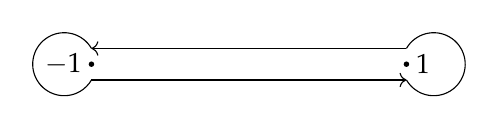
\begin{tikzpicture}[scale=1, transform shape]
        \fill (-2,0) circle (1pt);
        \fill (2,0) circle (1pt);
        \node [left] at (-2,0) {$-1$};
        \node [right] at (2,0) {$1$};
        \draw (2,0.2) arc (150:-150:0.4);
        \draw (-2,0.2) arc (30:330:0.4);
        \draw[->] (2,0.2) -- (-2,0.2);
        \draw[->] (-2,-0.2) -- (2,-0.2);
    \end{tikzpicture}
    \end{center}
    \caption{Contour $\gamma_{\ep, \delta}$}%
    \label{fig:}
    \end{figure}
    with radius $\ep$ and width $\delta$. Then $\int_{\gamma} = \int_{\gamma_{\ep, \delta}}$. Then we have
    \begin{align*} 
        \lim_{\ep, \delta \to 0} \int_{\gamma_{\ep, \delta}} \sqrt{z^2-1} \dd{z} &= \int_{-1}^1 i \cdot \sqrt{1-x^2} \dd{x}+ \int_{-1}^1 -i \sqrt{1-x^2} \dd{x} \\
                                                                                 &= -2i \int_{-1}^1 \sqrt{1-x^2} \dd{x} = -\pi i.
    \end{align*}

    Alternatively, we may use the transformation $z = \frac{1}{2}$ to obtain
    \[ \int_{\abs{z} = 2} \sqrt{z^2-1} \dd{z} = \int_{\abs{w} = \frac{1}{2}} \frac{\sqrt{1-w^2}}{w^3} \dd{w} = 2 \pi i \Res_0 \frac{\sqrt{1-w^2}}{w^3} = 2 \pi i \cdot \frac{-1}{2} = - \pi i. \]
\end{exm}

\begin{exm}
    Consider the contour $\gamma$ given by
    \begin{figure}[H]
    \begin{center}
    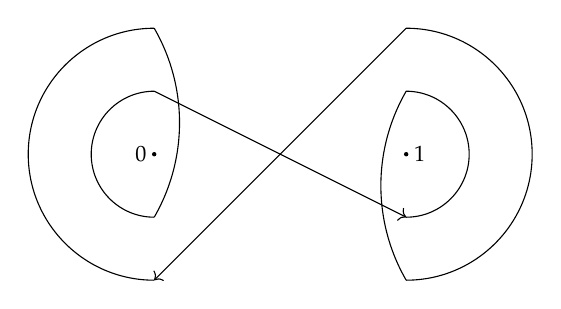
\begin{tikzpicture}[scale=0.8, transform shape]
        \draw (-2,-2) arc (270:90:2);
        \draw (-2,2) arc (30:-30:3);
        \draw (-2,-1) arc (270:90:1);
        \fill (-2,0) circle (1pt);
        \node [left] at (-2,0) {$0$};
        \draw[->] (-2,1) -- (2,-1);
        \draw (2,-1) arc (-90:90:1);
        \draw (2,1) arc (150:210:3);
        \draw (2,-2) arc (-90:90:2);
        \draw[->] (2,2) -- (-2,-2);
        \fill (2,0) circle (1pt);
        \node [right] at (2,0) {$1$};
    \end{tikzpicture}
    \end{center}
    \caption{Contour $\gamma$}%
    \label{fig:}
    \end{figure}
    Then we have 
    \begin{align*} 
        \int_{\gamma} \frac{e^z-1}{z^2(z-1)} \dd{z} &= 2 \pi i (n(\gamma, 0) \Res_0 f + n(\gamma, 1) \Res_1 f) \\
                                                    &= 2 \pi i (-2(-1) + 2(e-1)) \\
                                                    &= 2 \pi i e.
    \end{align*}
\end{exm}


\section{Harmonic Functions}%
\label{sec:harmonic_functions}

We say $u \colon \Omega \to \R$ is \textit{harmonic} if it has continuous second partial derivatives and satisfies \textbf{Laplace's equation}
\[ \pdv[2]{u}{x} + \pdv[2]{u}{y} = 0. \]
Harmonic functions have applications in electricity and magnetism, fluid dynamics, gravity, and heat conduction.

\begin{lem}
    Let $f \colon \Omega \to \C$ be holomorphic and write $f(x+iy) = u(x,y) + iv(x,y)$. Then $u,v$ are harmonic.
\end{lem}

\begin{proof}
    By the Cauchy-Riemann equations, we have
    \[ \pdv[2]{u}{x} + \pdv[2]{u}{y} = \pdv{x} \pdv{v}{y} - \pdv{y} \pdv{v}{x} = 0 \]
    and similar for $v$.
\end{proof}

There is a converse to this.

\begin{thm}
    Let $\Omega \subset \C$ be simply connected and $u \colon \Omega \to \R$ be harmonic. Then there exists a holomorphic $f \colon \Omega \to \C$ such that $u = \Re(f)$. Moreover, $f$ is unique up to $f \rightsquigarrow f + ic$ for $c \in \R$.
\end{thm}

\begin{proof}
    Define $g \coloneqq \pdv{u}{u} - i \pdv{u}{y}$ and integrate. Then we see that $g$ is holomorphic because the components have continuous first derivatives and the Cauchy-Riemann equations are satisfied because $u$ is harmonic and by symmetry of mixed partials.

    Then because $\Omega$ is simply connected, there exists a primitive $f \colon \Omega \to \C$ such that $f' = g$. Now write $f = \wt{u} + i \wt{v}$ and note that 
    \begin{align*} 
        f' &= \pdv{\wt{u}}{x} + i \pdv{\wt{v}}{x} = \pdv{\wt{u}}{x} - i \pdv{\wt{u}}{y} \\
           &= g = \pdv{u}{x} - i \pdv{u}{y}. 
    \end{align*}
    Therefore $\wt{u} = u + a$ for some $a \in \R$, so up to $f \rightsquigarrow f - a$, we have $\Re(f) = u$.

    To show uniqueness, note that if $f_1, f_2$ are two such functions, then $\Re(f_1 - f_2) = 0$ and thus $f_1 - f_2 \in i\R$. But this implies that $\Omega$ is sent to something that is not open so $f_1 - f_2$ is a constant.
\end{proof}

\begin{thm}
    Let $u \colon \Omega \to \R$ be harmonic. Then for all $z \in \Omega, r \in \R_{>0}$ such that $\ol{D}(z,r) \subset \Omega$, we have
    \[ u(z) = \frac{1}{2 \pi} \int_0^{2 \pi} u(z + re^{i\theta}) \dd{\theta}. \]
\end{thm}

\begin{proof}
    There exists $D = D(z, r') \subset \Omega$ for $r' > r$ and $f$ holomorphic on $D$ such that $\eval{u}_D = \Re(f)$. Applying the Cauchy integral formula, we have
    \[ f(z) = \frac{1}{2 \pi i} \int_{\partial D(z, r)} \frac{f(w)}{z-w} \dd{w} = \frac{1}{2 \pi i} \int_0^{2 \pi} \frac{f(z+ re^{i\theta})}{re^{i\theta}} ire^{i\theta} \dd{\theta} = \frac{1}{2\pi} \int_0^{2\pi} f(z+re^{i\theta}) \dd{\theta}. \]
    Now the desired result follows by taking real parts.
\end{proof}

\begin{thm}[Maximum principle for harmonic functions]
    Let $u$ be harmonic on a connected $\Omega \subset \C$. Then if $u$ has a maximum in $\Omega$, then $u$ is constant.
\end{thm}

\begin{proof}
    If $\Omega$ is simply connected, then we know $u$ is the real part of some holomorphic $f$, so using the maximum principle for $g = e^f$, we obtain the desired result. In general, suppose $u$ has a maximum $c$ at a point $z_0 \in \Omega$. Then for $z_0 \in D \subset \Omega$ we know $u$ is constant on $D$. Now define $U = \qty{z \in \Omega \mid u \equiv c \text{ near }z}$. By definition, $U$ is open, but $U$ is also closed in $\Omega$, so $U = \Omega$.
\end{proof}

\begin{exm}
    The function $u(x,y) = \log(\sqrt{x^2 + y^2}) \colon \R^2 \setminus \qty{(0,0)} \to \R$ is harmonic.
\end{exm}

\begin{cor}
    Let $\Omega \subset \C = \R^2$ be bounded. Suppose $u_1, u_2 \colon \ol{\Omega} \to \R$ are continuous on $\ol{\Omega}$ and harmonic on $\Omega$. Further suppose that $u_1 = u_2$ on $\partial \Omega$. Then $u_1 = u_2$.
\end{cor}

\begin{proof}
    Write $u = u_1 - u_2$. We know $u = 0$ on $\partial \Omega$ and is harmonic on $\Omega$ and continuous on $\ol{\Omega}$. By the maximum principle, if $u$ has a max in $\Omega$ then it is constant, but we know $u$ attains a maximum on $\ol{\Omega}$ Therefore $u \leq 0$. Applying the same reasoning to $-u$, we see that $u \geq 0$.
\end{proof}

Now we would like to study the Dirichlet problem. Given $\Omega \subset \C = \R^2$ and $g \colon \partial \Omega \to \R$ continuous, we want to find $u \colon \ol{\Omega} \to \R$ continuous on $\ol{\Omega}$ and harmonic on $\Omega$ such that $\eval{u}_{\partial \Omega} = g$.

\begin{exm}
    Let $\Omega = A = \qty{z \in \C \mid R_1 < \abs{z} < R_2}$ and set $u(z) = 0$ if $\abs{z} = R_1$ and $u(z) = 1$ when $\abs{z} = R_2$. Then the Laplace equation is a linear PDE and we expect $u = u(r) = u(\sqrt{x^2+y^2})$. In fact, we can set
    \[ u = \frac{\log \sqrt{x^2 + y^2} - \log R_1}{\log R_2 - \log R_1}. \]
\end{exm}

Now the generalized Dirichlet problem is as follows: Suppose $\Omega$ is simply connected with piecewise smooth boundary. Then the Riemann mapping theorem gives us a holomrophic bijection $F \colon \Omega \to D$. Then this extends to a homeomorphism $\ol{F} \colon \ol{\Omega} \to \ol{D}$. Now fix a finite set $S \subset \partial \Omega$ and continuous $g \colon \partial \Omega \setminus S \to \R$. 

\begin{prob}[Generalized Dirichlet problem]
    Find a continuous function $u \colon \ol{\Omega} \setminus S \to \R$ that is harmonic on $\Omega$ such that $\eval{u}_{\partial \Omega \setminus S} = g$. Note that if such a $u$ exists, then it is unique.
\end{prob}

\begin{exm}
    Let $\Omega = \mc{H}$, $S = 0$, and set $g(x) = \begin{cases}
        1 & x < 0 \\
        0 & x > 0.
    \end{cases}$
    \begin{figure}[H]
    \begin{center}
    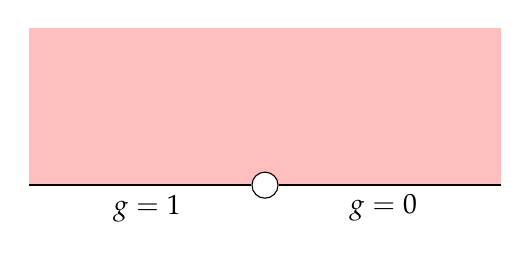
\begin{tikzpicture}[scale=1, transform shape]
        \fill[pink] (-3,0) rectangle (3,2);
        \node [circle, draw=black, fill=white, minimum size=1pt] (O) at (0,0) {};
        \draw[thick] (O) -- (-3,0);
        \draw[thick] (O) -- (3,0);
        \node[below] at (1.5,0) {$g=0$};
        \node[below] at (-1.5,0) {$g=1$};
    \end{tikzpicture}
    \end{center}
    \caption{Generalized Dirichlet problem on upper half plane.}%
    \label{fig:}
    \end{figure}
    Then we take $u = \frac{\arg(z)}{\pi}$.
\end{exm}

\begin{exm}
    Consider the generalized Dirichlet problem given by
    \begin{figure}[H]
    \begin{center}
    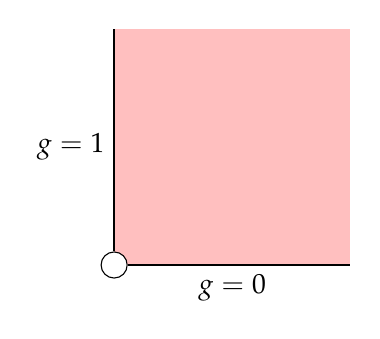
\begin{tikzpicture}[scale=1, transform shape]
        \fill[pink] (0,0) rectangle (3,3);
        \node [circle, draw=black, fill=white, minimum size=1pt] (O) at (0,0) {};
        \draw[thick] (O) -- (0,3);
        \draw[thick] (O) -- (3,0);
        \node[below] at (1.5,0) {$g=0$};
        \node[left] at (0,1.5) {$g=1$};
    \end{tikzpicture}
    \end{center}
    \caption{Generalized Dirichlet problem on first quadrant.}%
    \label{fig:}
    \end{figure}
    Then we may take $u = \frac{2}{\pi} \arg(z)$.
\end{exm}

\begin{lem}
    Let $f \colon \Omega_2 \to \Omega_1$ be holomorphic and $u_1 \colon \Omega_1 \to \R$ be harmonic. Then $u_2 = u_1 \circ f$ is harmonic.
\end{lem}

\begin{proof}
    Locally, we can write $u_1 = \Re(g)$ for some holomorphic $g$. Then $u_2 = \Re(g \circ f)$ must be harmonic.
\end{proof}

\begin{exm}
    Consider $\Omega = \qty{z \mid \abs{z} < 1}$ and $S = \qty{1, i}$.
    \begin{figure}[H]
    \begin{center}
    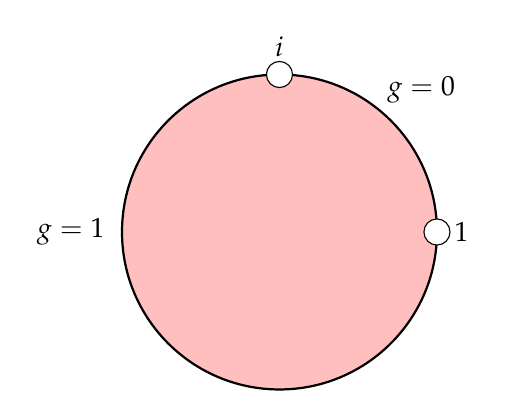
\begin{tikzpicture}[scale=1, transform shape]
        \fill [pink] (0,0) circle (2);
        \draw[thick] (2,0) arc (0:90:2);
        \draw[thick] (0,2) arc (90:360:2);
        \node [circle, draw=black, fill=white, minimum size=1pt] (o) at (2,0) {};
        \node [circle, draw=black, fill=white, minimum size=1pt] (i) at (0,2) {};
        \node[right] at (2.1,0) {$1$};
        \node[above] at (0,2.1) {$i$};
        \node at (1.8,1.8) {$g=0$};
        \node[left] at (-2.1,0) {$g=1$};
    \end{tikzpicture}
    \end{center}
    \caption{Generalized Dirichlet problem on disk}%
    \label{fig:}
    \end{figure}
    Then a M\"obius transformation $f \colon \P^1 \to \P^1$ taking $D \to \mc{H}$ and $1, i, -1 \mapsto \infty, 0, 1$ is given by
    \[ f(z) = \frac{z-i}{z-1} \frac{-1-1}{-1-i} = \frac{z-i}{z-1} \frac{2}{1+i}, \]
    so we may take
    \begin{align*} 
        u(z) &= (1 - \frac{1}{\pi} \arg \qty(\frac{z-i}{z-1} \frac{2}{1+i})) \\ 
             &= 1 - \frac{1}{\pi} (\arg(1-i) + \arg(z-i) -\arg(z-1)) \\ 
             &= \frac{5}{4} - \frac{1}{\pi} (\arg(z-i) - \arg(z-1)). 
    \end{align*}
\end{exm}

Now we will give a general solution of the Dirichlet problem for the disk. Recall the mean value property
\[ u(0) = \frac{1}{2\pi} \int_0^{2\pi} u(re^{i\theta}) \dd{\theta} \]
for $0 < r < 1$. Assume that $u$ extends continuously to $\ol{D} \setminus S$ and is bounded. Then as $r \to 0$, we see that $u(0) = \frac{1}{2\pi} \int_0^{2\pi} u(e^{i\theta}) \dd{\theta}$. Now we use the Blaschke factor 
\[ \psi_z \colon D \xrightarrow{\sim} D \qquad w \mapsto \frac{z-w}{1-\ol{z}w}. \]
Then if $\wt{u} = u \circ \psi_z$, we have
\begin{align*}
    u(z) &= \wt{u}(0) \\
         &= \frac{1}{2\pi} \int_0^{2\pi} \wt{u}(e^{i\phi}) \dd{\phi} \\
         &= \frac{1}{2\pi} \int_{\abs{v}=1} \wt{u}(v) \dd{(\arg v)} \\
         &= \frac{1}{2\pi} \int_{\abs{v}=1} \wt{u}(v) \frac{1}{i} \frac{\dd{v}}{v} \\
         &= \frac{1}{2\pi} \int_{\abs{w}=1} u(w) \frac{1-\abs{z}^2}{\abs{w-z}^2} \frac{1}{i} \frac{\dd{w}}{w} \\
         &= \frac{1}{2\pi} \int_0^{2\pi} u(re^{i\phi}) \frac{1-r^2}{1+r^2-2r\cos(\theta-\phi)} \dd{\phi}
\end{align*}
Because we have
\begin{align*}
    \frac{\dd{v}}{v} &= \frac{\dd{(z-w)}}{z-w} - \frac{\dd{(1-\ol{z}w)}}{1-\ol{z}w} \\
                     &= \dd{w} \qty(\frac{-1}{z-2} + \frac{\ol{z}}{z-\ol{z}w}) \\
                     &= \dd{w} \qty(\frac{{-1 + \ol{z}\ol{w} + z \ol{z} - w \ol{z}}}{(z-w)(1-\ol{z}w)}) \\
                     &= \frac{\dd{w}}{w} \qty(\frac{-1 + \abs{z}^2}{(z-w)(\ol{w}-\ol{z})}) \\
                     &= \frac{\dd{w}}{w} \frac{1-\abs{z}^2}{\abs{w-z}^2}.
\end{align*}

Now if $\Omega$ is simply connected, we have $\ol{F} \colon \ol{\Omega} \xrightarrow{\sim} \ol{D}$ that restricts to a holomorphic bijection $F \colon \Omega \xrightarrow{\sim} D$. Then if $\wt{u} \colon D \to \R$ is a solution on $D$, $\wt{u} \circ \ol{F}$ is a solution on $\Omega$.








\end{document}
